% This is "sig-alternate.tex" V2.1 April 2013
% This file should be compiled with V2.5 of "sig-alternate.cls" May 2012
%
% This example file demonstrates the use of the 'sig-alternate.cls'
% V2.5 LaTeX2e document class file. It is for those submitting
% articles to ACM Conference Proceedings WHO DO NOT WISH TO
% STRICTLY ADHERE TO THE SIGS (PUBS-BOARD-ENDORSED) STYLE.
% The 'sig-alternate.cls' file will produce a similar-looking,
% albeit, 'tighter' paper resulting in, invariably, fewer pages.
%
% ----------------------------------------------------------------------------------------------------------------
% This .tex file (and associated .cls V2.5) produces:
%       1) The Permission Statement
%       2) The Conference (location) Info information
%       3) The Copyright Line with ACM data
%       4) NO page numbers
%
% as against the acm_proc_article-sp.cls file which
% DOES NOT produce 1) thru' 3) above.
%
% Using 'sig-alternate.cls' you have control, however, from within
% the source .tex file, over both the CopyrightYear
% (defaulted to 200X) and the ACM Copyright Data
% (defaulted to X-XXXXX-XX-X/XX/XX).
% e.g.
% \CopyrightYear{2007} will cause 2007 to appear in the copyright line.
% \crdata{0-12345-67-8/90/12} will cause 0-12345-67-8/90/12 to appear in the copyright line.
%
% ---------------------------------------------------------------------------------------------------------------
% This .tex source is an example which *does* use
% the .bib file (from which the .bbl file % is produced).
% REMEMBER HOWEVER: After having produced the .bbl file,
% and prior to final submission, you *NEED* to 'insert'
% your .bbl file into your source .tex file so as to provide
% ONE 'self-contained' source file.
%
% ================= IF YOU HAVE QUESTIONS =======================
% Questions regarding the SIGS styles, SIGS policies and
% procedures, Conferences etc. should be sent to
% Adrienne Griscti (griscti@acm.org)
%
% Technical questions _only_ to
% Gerald Murray (murray@hq.acm.org)
%
% Technical questions related to COCO/BBOB to bbob@lri.fr
% ===============================================================
%
% For tracking purposes - this is V2.0 - May 2012

\documentclass{sig-alternate}

\usepackage{graphicx}
\usepackage{rotating}
\usepackage[dvipsnames]{xcolor}  % color is sufficient
%\usepackage[hidelinks]{hyperref} % make COCO papers clickable
\pdfpagewidth=8.5in
\pdfpageheight=11in
\special{papersize=8.5in,11in}

\renewcommand{\topfraction}{1}	% max fraction of floats at top
\renewcommand{\bottomfraction}{1} % max fraction of floats at bottom
% Parameters for TEXT pages (not float pages):
\setcounter{topnumber}{3}
\setcounter{bottomnumber}{3}
\setcounter{totalnumber}{3}     % 2 may work better
\setcounter{dbltopnumber}{4}    % for 2-column pages
\renewcommand{\dbltopfraction}{1}	% fit big float above 2-col. text
\renewcommand{\textfraction}{0.0}	% allow minimal text w. figs
% Parameters for FLOAT pages (not text pages):
\renewcommand{\floatpagefraction}{0.80}	% require fuller float pages
% N.B.: floatpagefraction MUST be less than topfraction !!
\renewcommand{\dblfloatpagefraction}{0.7}	% require fuller float pages

%%%%%%%%%%%%%%%%%%%%%%%%%%%%%%%%%%%%%%%%%%%%%%%%%%%%%%%%%%%%%%%%%%%%%%%%%%%%%%%
%%%%%%%%% TO BE EDITED %%%%%%%%%%%%%%%%%%%%%%%%%%%%%%%%%%%%%%%%%%%%%%%%%%%%%%%%
%%%%%%%%%%%%%%%%%%%%%%%%%%%%%%%%%%%%%%%%%%%%%%%%%%%%%%%%%%%%%%%%%%%%%%%%%%%%%%%
% rungeneric.py writes data into a subfolder of ppdata
\newcommand{\bbobdatapath}{ppdata/} % default output folder of rungeneric.py
\input{\bbobdatapath bbob_pproc_commands.tex} % provide default of algname and algfolder
\renewcommand{\algname}{IBEA}  % name of algorithm as it should appear in the text
 \renewcommand{\algfolder}{ibea_epsilon_python/} % subfolder of \bbobdatapath for processed algorithm
% Find all \change commands in the text below and update the information according to your data
%%%%%%%%%%%%%%%%%%%%%%%%%%%%%%%%%%%%%%%%%%%%%%%%%%%%%%%%%%%%%%%%%%%%%%%%%%%%%%%

\graphicspath{{\bbobdatapath\algfolder}}

\newcommand{\DIM}{\ensuremath{\mathrm{DIM}}}
\newcommand{\aRT}{\ensuremath{\mathrm{aRT}}}
\newcommand{\FEvals}{\ensuremath{\mathrm{FEvals}}}
\newcommand{\nruns}{\ensuremath{\mathrm{Nruns}}}
\newcommand{\Dfb}{\ensuremath{\Delta f_{\mathrm{best}}}}
\newcommand{\Df}{\ensuremath{\Delta f}}
\newcommand{\nbFEs}{\ensuremath{\mathrm{\#FEs}}}
\newcommand{\hvref}{\ensuremath{HV_\mathrm{ref}}}
\newcommand{\fopt}{\hvref}
%\newcommand{\fopt}{\ensuremath{f_\mathrm{opt}}}
\newcommand{\ftarget}{\ensuremath{f_\mathrm{t}}}
\newcommand{\CrE}{\ensuremath{\mathrm{CrE}}}
\newcommand{\change}[1]{{\color{red} #1}}
\newcommand{\TODO}[1]{{\color{orange} !!! #1 !!!}}

% To suppress warnings about PDF page groups:
%\pdfsuppresswarningpagegroup=1     % Dimo: gives errors on my machine

%%%%%%%%%%%%%%%%%%%%%%   END OF PREAMBLE   %%%%%%%%%%%%%%%%%%%%%%%%%%%%%%%%%%%%

\begin{document}
%
% --- Author Metadata here ---
%\conferenceinfo{GECCO'17,} {July 20-24, 2017, Denver, CO, USA.}
%\CopyrightYear{2016}
%\crdata{TBA}
%\clubpenalty=10000
%\widowpenalty = 10000
% --- End of Author Metadata ---

\title{Benchmarking of the Indicator-based evolution algorithm using the Bi-Objective BBOB Test Suite
% \titlenote{If needed}
}
\subtitle{Final report
\titlenote{Submission deadline: October 21st.}}
% Camera-ready paper due by May 4th.

%
% You need the command \numberofauthors to handle the 'placement
% and alignment' of the authors beneath the title.
%
% For aesthetic reasons, we recommend 'three authors at a time'
% i.e. three 'name/affiliation blocks' be placed beneath the title.
%
% NOTE: You are NOT restricted in how many 'rows' of
% "name/affiliations" may appear. We just ask that you restrict
% the number of 'columns' to three.
%
% Because of the available 'opening page real-estate'
% we ask you to refrain from putting more than six authors
% (two rows with three columns) beneath the article title.
% More than six makes the first-page appear very cluttered indeed.
%
% Use the \alignauthor commands to handle the names
% and affiliations for an 'aesthetic maximum' of six authors.
% Add names, affiliations, addresses for
% the seventh etc. author(s) as the argument for the
% \additionalauthors command.
% These 'additional authors' will be output/set for you
% without further effort on your part as the last section in
% the body of your article BEFORE References or any Appendices.

\numberofauthors{5} %  in this sample file, there are a *total*
% of EIGHT authors. SIX appear on the 'first-page' (for formatting
% reasons) and the remaining two appear in the \additionalauthors section.
%
\author{
% You can go ahead and credit any number of authors here,
% e.g. one 'row of three' or two rows (consisting of one row of three
% and a second row of one, two or three).
%
% The command \alignauthor (no curly braces needed) should
% precede each author name, affiliation/snail-mail address and
% e-mail address. Additionally, tag each line of
% affiliation/address with \affaddr, and tag the
% e-mail address with \email.
%
% 1st. author
 %\titlenote{Dr.~Trovato insisted his name be first.}\\
%       \affaddr{Institute for Clarity in Documentation}\\
%       \affaddr{1932 Wallamaloo Lane}\\
%       \affaddr{Wallamaloo, New Zealand}\\
%       \email{trovato@corporation.com}
%% 2nd. author
 %\titlenote{The secretary disavows
%any knowledge of this author's actions.}\\
%       \affaddr{Institute for Clarity in Documentation}\\
%       \affaddr{P.O. Box 1212}\\
%       \affaddr{Dublin, Ohio 43017-6221}\\
%       \email{webmaster@marysville-ohio.com}
%% 3rd. author
\alignauthor Daro Heng %\titlenote{This author is the
%one who did all the really hard work.}\\
%       \affaddr{The Th{\o}rv{\"a}ld Group}\\
%       \affaddr{1 Th{\o}rv{\"a}ld Circle}\\
%       \affaddr{Hekla, Iceland}\\
%       \email{larst@affiliation.org}
%\and  % use '\and' if you need 'another row' of author names
%% 4th. author
\alignauthor
Karim Kouki
\alignauthor
Ahmed Mazari
\and
\alignauthor Mihaela Sorostinean
%       \affaddr{Brookhaven Laboratories}\\
%       \affaddr{Brookhaven National Lab}\\
%       \affaddr{P.O. Box 5000}\\
%       \email{lleipuner@researchlabs.org}
%% 5th. author
\alignauthor Aris Tritas
%       \affaddr{NASA Ames Research Center}\\
%       \affaddr{Moffett Field}\\
%       \affaddr{California 94035}\\
%       \email{fogartys@amesres.org}
}

\maketitle
\begin{abstract}
The objective of this project was to study, implement and benchmark the Indicator Based Evolutionary Algorithm (IBEA) using  the Comparing Continuous Optimizer (COCO) platform. Firstly, a brief presentation of evolution strategies and the algorithm is provided. Secondly, our implementation and experimental setup is described. Finally, we discuss the obtained results and compare them to both baseline approaches and related work.
\end{abstract}

% Add any ACM category that you feel is needed, not mandatory anymore
%\category{G.1.6}{Numerical Analysis}{Optimization}[global optimization,
%unconstrained optimization]
%\category{F.2.1}{Analysis of Algorithms and Problem Complexity}{Numerical Algorithms and Problems}

% Complete with anything that is needed
\terms{Algorithms}

% Complete with anything that is needed
\keywords{Benchmarking, Black-box optimization, Bi-objective optimization}

\section{Setting}
In the context of a multi-objective optimization, the main goal is to find a good approximation of the set of Pareto-optimal solutions.
An evolutionary algorithm is an exploration strategy of the domain space $\mathbb{R}^d$ which seeks optimal solution vectors defined in $\mathbb{R}^2$.

The input of the algorithm is the size of the population ($\alpha$), and a fitness scaling factor ($\kappa$). The output of the algorithm is an approximation of the Pareto-set.

The performance measure used by IBEA for the optimization goal is a binary indicator of the relative quality of two solution vectors sets in the Pareto objective space. Likewise, this indicator is defined for pairwise comparisons of solution vectors. The epsilon indicator reduces the minimum distance to improve on the Pareto set approximation to a single scalar. Intuitively, this may incur a  loss of information with respect to each dimension of the multi-objective optimization. Indeed, we are required to choose the minimum distance of improvement across all objectives. However, this means that we may miss on potential improvement on a specific axis.

The fitness of an approximation set is defined as a dominance preserving relation, and is computed with the epsilon indicator function.
$$ F(x^1) = \sum_{x^2 \in P \setminus \{x^1\}} - \exp{\frac{I(\{x^1\}, \{x^2\})}{\kappa}}$$
The domain space typically has axes with different scales. Therefore, Adaptive-IBEA scales the objective function values as well as the range of values taken by the indicator function. This scheme decreases the need parameter tuning in face of problem and indicator function diversity.
 
\textbf{Remark} detail about the dominance preserving relation

\section{Implementation}
As far as the implementation in Python is concerned we chose to represent the population in a compact data structure and did all numerical computation with NumPy. The steps of the algorithm were inlined in a single optimization function, except for the recombination and mutation operators which were implemented in separate functions to achieve modularity during testing.

Python dictionary, grid search

\section{Experiments}
\subsection{La galere}
 For the first part of the project our milestone was to have a working version of the algorithm, and potentially reasonable results on at least some groups of functions.
 
Without further changes to the original strategy, our algorithm does not seem to reach the optimal Pareto set of solution vectors. We tried applying recombination and mutation with high and low probabilities respectively, following the literature. This did not yield improved results, which leads us to think that either our implementation lacks robustness, or has a subtle bug.

We intended to:
\begin{enumerate}
\item Experiment with self-adaptive strategies for the mutation step, and 
\item Implement Self-Adaptive SBX which seeks an optimal index for the approximation distribution used
\end{enumerate}
\subsection{Setup}
The proposed implementation of the IBEA algorithm was tested with the collection of benchmark problems comprised in the COCO platform. We performed several experiments with various combinations of parameters in order to evaluate the influence of specific parameters on the results for different categories of benchmark problems. Therefore we varied the following parameters:
\begin{itemize}
\item The budget - various values between 300, 500, 750, 850, 1000
\item Population size - varied between 50, 60, 80, 100, 200
\item Number of offspring - 20, 30 or 40
\item Mutation probability - 0.7, 0.8, 0.9, 1.0
\item Recombination probability - or probability of crossover for the recombination step - 0.4, 0.6, 0.8, 0.9, 1.0
\item Variance - 1.3 , 2.5, 5, 10, 15
\item Offspring : - 20, 30, 35, 40
\item Dimension : 2, 5, 10, 20, 40
\item Max iterations: $10^6$, $10^9$
\item Distribution index for the SBX operator: 2, 5 or 20 (the value suggested by the authors)
\item Operators : Isotropic, Derandomized
\end{itemize}

Since the number of variable parameters was considerable, carrying experiments with all combinations between them was impossible, so we selected a limited number of combinations which we considered might give significant results. The sets of parameters that we used in our experiments are illustrated in table 1.  
Running a bi-objective algorithm in a laptop is not an easy task. It's both time and RAM consuming.  The execution takes from 5 to 23 hours to finish with a budget of 1000. The timing experiment  is intrinsically associated with the size of the population and the dimension. 
For that reason, we tried only one configuration for 40 dimensions that took almost 48h  with a moderate budget of 300.  
In order to try several parameterizations of the algorithm we  were obliged to make non stopping running of the algorithm on different machine with different parameter in order to evaluate how  the algorithm performs under different parameterizations. We conclude from this empirical study that a high variance and low variance impacts negatively the performance of the algorithm. The trick is to find a trade-off between the size of population, variance and the recombination values.

\subsection{Recombination}

The operator we used were intermediate weighting, discrete recombination  and finally, the Simulated Binary Crossover \cite{deb1994simulated}. However, results using these operators were not encouraging. The reason for that may be a rather naive exploration of the search space.

In this case, the Simulated Binary Operator was chosen for the recombination part.
\subsection{Variation}

For the mutation step, we simply added isotropic Gaussian noise with fixed variance to the produced offspring. However, it is well known that fixing variance does not speed up search optimally.
a polynomial distribution was used for the mutation part.  
%%%%%%%%%%%%%%%%%%%%%%%%%%%%%%%%%%%%%%%%%%%%%%%%%%%%%%%%%%%%%%%%%%%%%%%%%%%%%%%
\section{CPU Timing}
%%%%%%%%%%%%%%%%%%%%%%%%%%%%%%%%%%%%%%%%%%%%%%%%%%%%%%%%%%%%%%%%%%%%%%%%%%%%%%%
% note that the following text is just a proposal and can/should be changed to your needs:
In order to evaluate the CPU timing of the algorithm, we have run the \algname with restarts on the entire bbob-biobj test suite \cite{biobj2016func} for $2 D$ function evaluations. The Python code was run on a Intel(R) Core(TM) i5-2400S CPU @ 2.50GHz with 4 processors and 8 cores. The time per function evaluation for dimensions 2, 3, 5, 10, 20 equals $1.7e{-3}$, $1.9e{-3}$, $2.0e{-3}$, $2.2e{-3}$, $2.4e{-3}$ seconds respectively.  


%%%%%%%%%%%%%%%%%%%%%%%%%%%%%%%%%%%%%%%%%%%%%%%%%%%%%%%%%%%%%%%%%%%%%%%%%%%%%%%
\section{Results}
%%%%%%%%%%%%%%%%%%%%%%%%%%%%%%%%%%%%%%%%%%%%%%%%%%%%%%%%%%%%%%%%%%%%%%%%%%%%%%%

Results of \algname\ from experiments according to \cite{hansen2016exp} and \cite{brockhoff2016biobjective} on the benchmark
functions given in \cite{biobj2016func} are presented in
Figures~\ref{fig:ECDFsingleOne}, \ref{fig:ECDFsingleTwo}, \ref{fig:ECDFsingleThree}, and \ref{fig:ECDFsGroups}, and in
Table~\ref{tab:aRTs}. The experiments were performed with COCO \cite{hansen2016cocoplat}, version 1.0.1, the plots were produced with version 1.0.4.
\subsection{Comparison of isotropic and derandomized mutation operators}
Derandomized mutation performs better on the following functions: (initial variance is 5, mutation prob is 0.8, crossover is  SBX-5 and Pr(0.8))
\begin{itemize}
\item Rosenbrock function 28.
\item Function 23
\item Much better on functions 26 \& 34
\item Function 2
\end{itemize}
By using $\alpha = 80$ and offsprings 30, better results were obtained for the following functions:
\begin{itemize}
\item function 13 (as well as function 12)
\item function 16
\item function 19
\item 2-moderate 4-multi-modal:  no good results in function group overall except for a slight improvement with this configuration on function 25
\end{itemize}

Function 15: Isotropic : Variance of 5 better than variance of 10, 
			 Derandomized: Smaller population as good as isotropic with small variance
			 
\subsubsection*{1-separable 2-moderate (3d)}: 
low mutation (0.1) is better for functions 12 and 13 and/or high recombination probability (>=0.8) is bad (why?)

smaller initial variance (3) is better for f13

\subsubsection*{1-separable 4-multi-modal} : high variance (10) is bad

\subsubsection*{1-separable 5-weakly-structured}
function 18: High recombination probability (0.7-0.9)
			  High mutation probability (around 0.7-0.8)  (along with isotropic pop 100)
			  High variance is bad

\subsubsection*{2-moderate 2-moderate}
Variance is a critical factor. 
Mutation with probability 1 without adaptation of the variance gives worse results.
Function 20 gives good results with mut0.3 in 5d - best mut0.3 recomb0.7 
28-2d as good for pop100 offs20 mut0.1 recomb0.7 var5.0 as for pop100 offs20 mut0.8 recomb0.6

\subsubsection*{2-moderate 5-weakly-structured}
Better results with low mutation probability (0.1-0.3)
Function 33: good results with relatively higher variance. Improved for a smaller population and moderate variance
26, 33: best with mut0.8 recomb0.6

\subsubsection*{3-ill-conditioned 3-ill-conditioned} 
variance is not the determinating factor. Isotropic a little worse.

Function 42: Derandomized and/or Higher population are better than pop=60

\subsubsection*{3-ill-conditioned 5-weakly-structured} 
High variance doesn't hurt w.r.t a smaller one. - 
Can't say much though because the problems are unstructured and hard)
f44-5d: mut0.8 recomb0.7 var5.0derandomized sbx2

\subsubsection*{4-multi-modal 4-multi-modal} 
Derandomized improves a tiny bit on isotropic.
\subsubsection*{4-multi-modal 5-weakly-structured}
 Function 48: high variance does not perform worse, on other functions of  derandomized is better
								    
Functions 54, 55: Can't say much. Derandomized/Smaller variance better.

Cases in which low mutation probability works:
2-moderate 5-weakly-structured: best is 0.3
3-ill-conditioned 5-weakly-structured: function 44 has good results

For 5-d space:
Function 53 performs very well with pop80, mut0.8, recombination1.0, derandomized
On the other hand it performs well with low mutation probability (0.1-0.3) on 3d
Find solutions really quick with var 3.

\subsection{aRT}
We observe with no surprise that our algorithm has a runtime of $1e{-3}$ iff the variance is adapted. gets to 10-3 on f12

We also observe that using a better indicator tends to find targets much faster.


%%%%%%%%%%%%%%%%%%%%%%%%%%%%%%%%%%%%%%%%%%%%%%%%%%%%%%%%%%%%%%%%%%%%%%%%%%%%%%%
%%%%%%%%%%%%%%%%%%%%%%%%%%%%%%%%%%%%%%%%%%%%%%%%%%%%%%%%%%%%%%%%%%%%%%%%%%%%%%%

% Scaling of ECDFs with dimension

%%%%%%%%%%%%%%%%%%%%%%%%%%%%%%%%%%%%%%%%%%%%%%%%%%%%%%%%%%%%%%%%%%%%%%%%%%%%%%%
\begin{figure*}
\centering
\begin{tabular}{@{\hspace*{-0.018\textwidth}}l@{\hspace*{-0.02\textwidth}}l@{\hspace*{-0.02\textwidth}}l@{\hspace*{-0.02\textwidth}}l@{\hspace*{-0.02\textwidth}}}
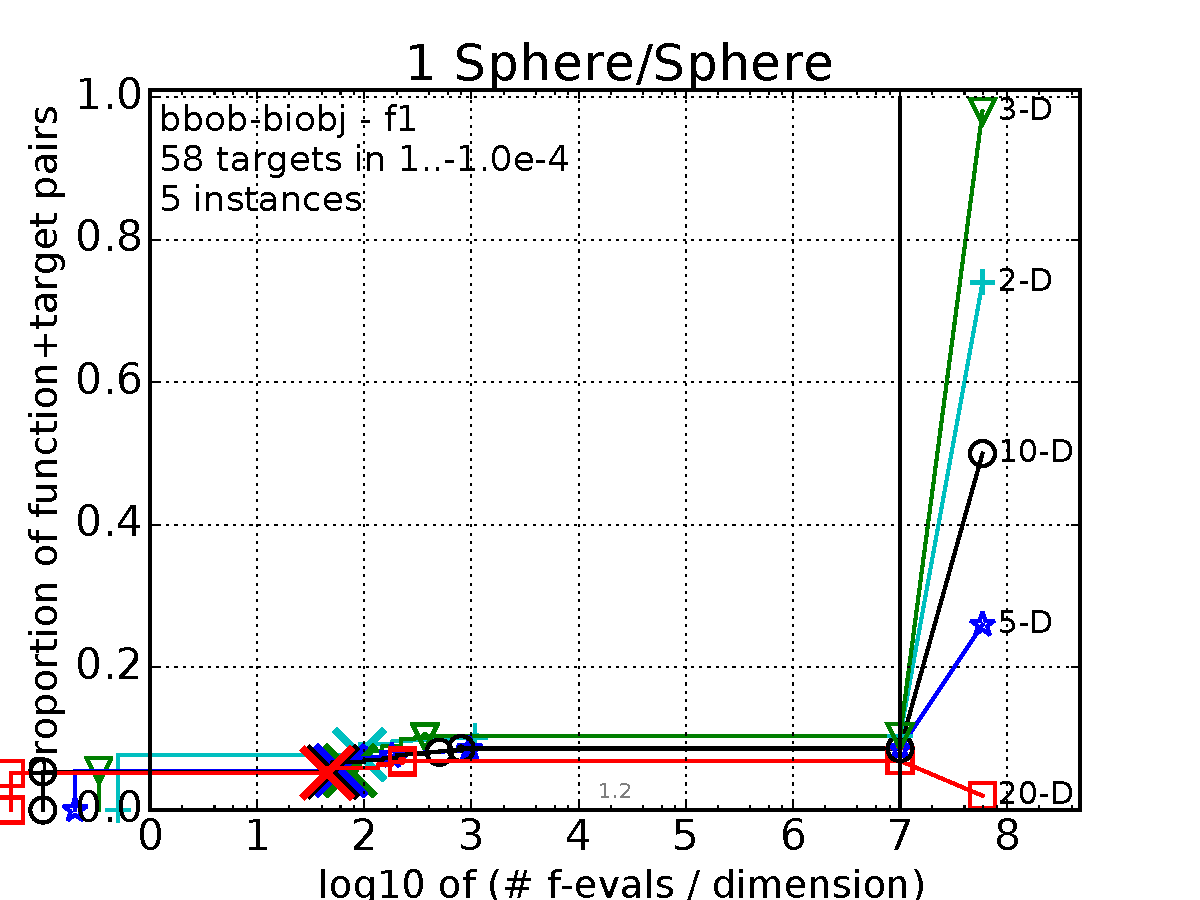
\includegraphics[width=0.25\textwidth]{pprldmany-single-functions/pprldmany_f001}&
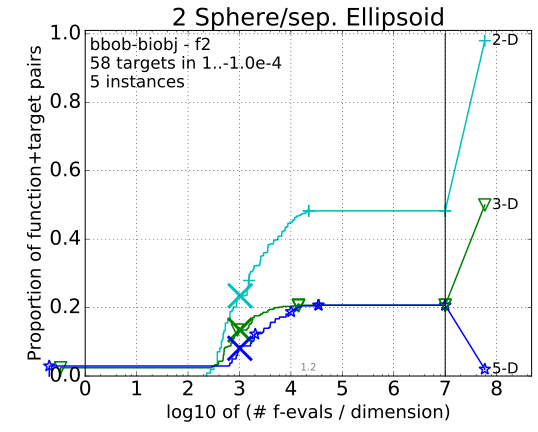
\includegraphics[width=0.25\textwidth]{pprldmany-single-functions/pprldmany_f002}&
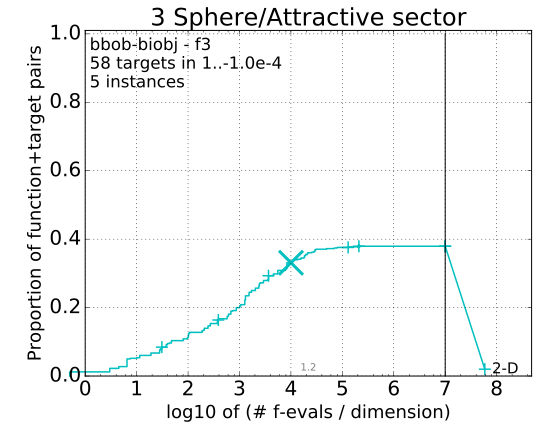
\includegraphics[width=0.25\textwidth]{pprldmany-single-functions/pprldmany_f003}&
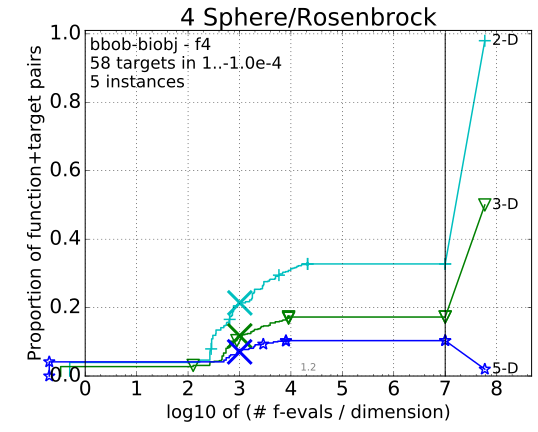
\includegraphics[width=0.25\textwidth]{pprldmany-single-functions/pprldmany_f004}\\[-1.8ex]
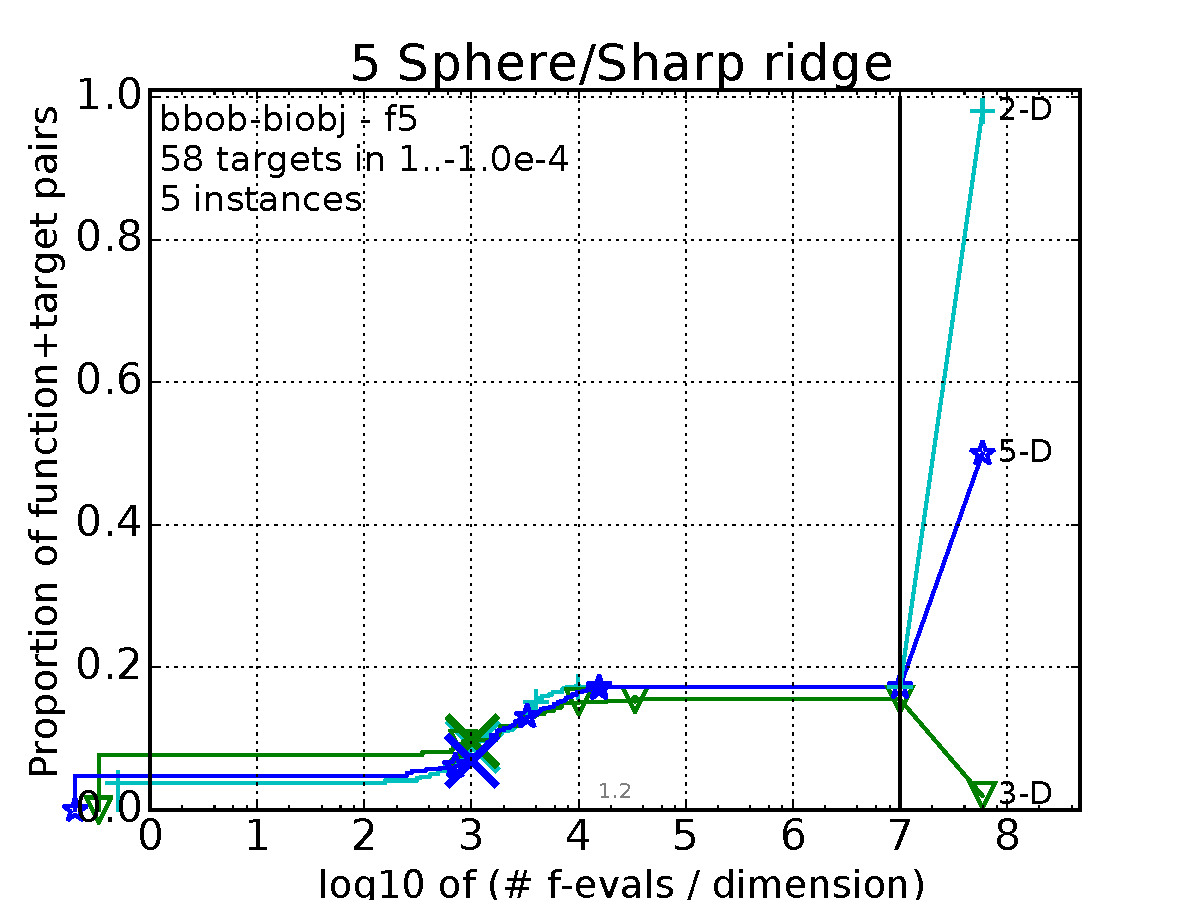
\includegraphics[width=0.25\textwidth]{pprldmany-single-functions/pprldmany_f005}&
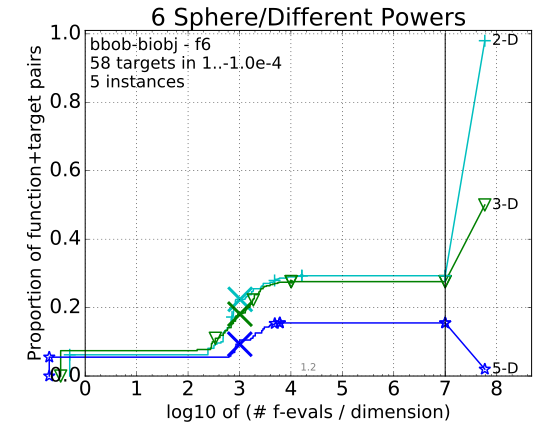
\includegraphics[width=0.25\textwidth]{pprldmany-single-functions/pprldmany_f006}&
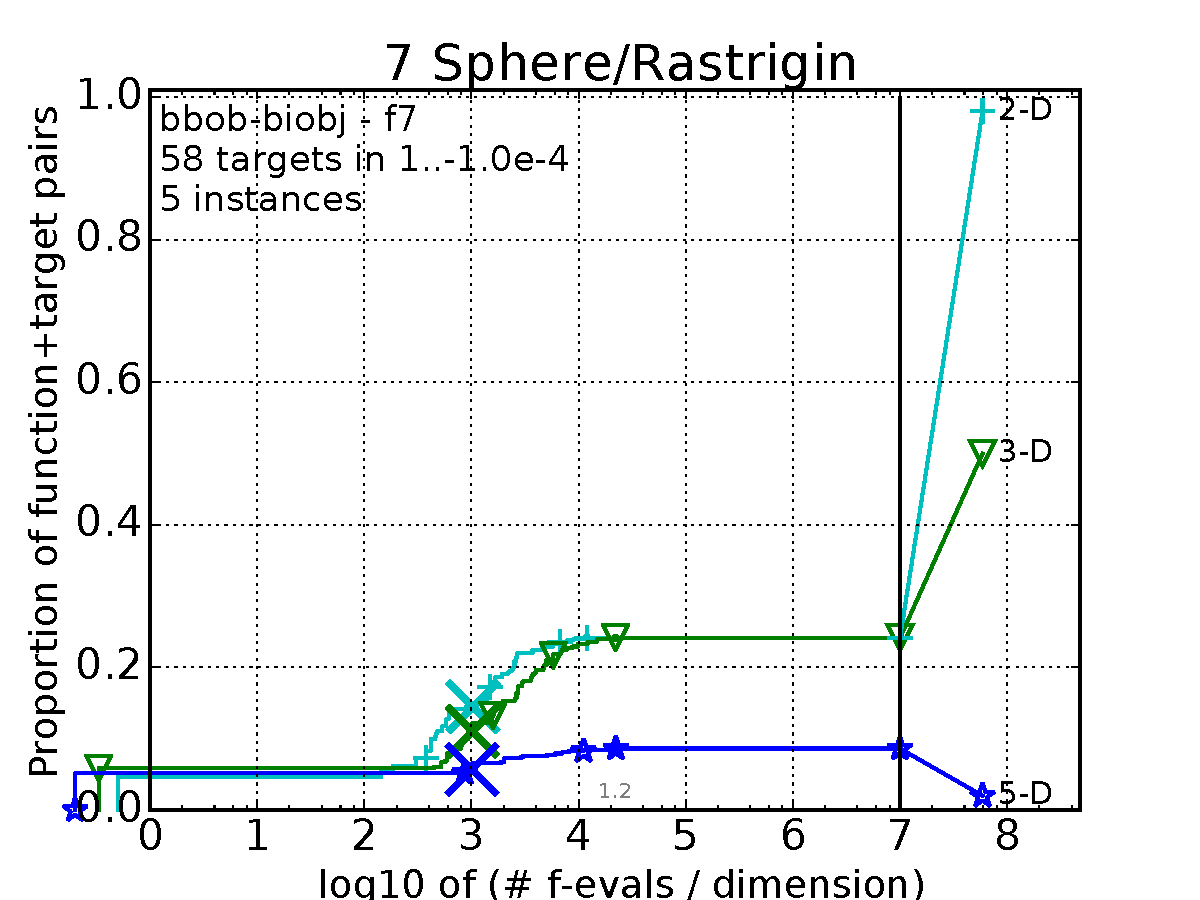
\includegraphics[width=0.25\textwidth]{pprldmany-single-functions/pprldmany_f007}&
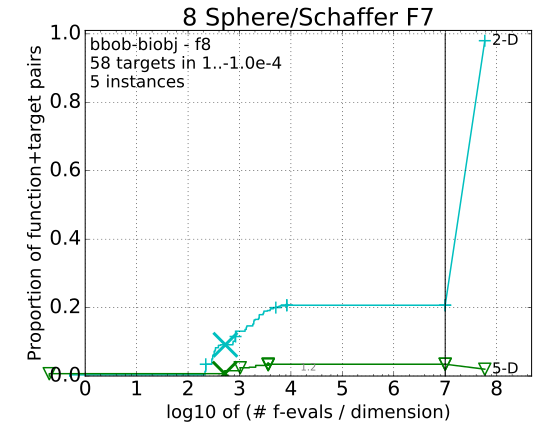
\includegraphics[width=0.25\textwidth]{pprldmany-single-functions/pprldmany_f008}\\[-1.8ex]
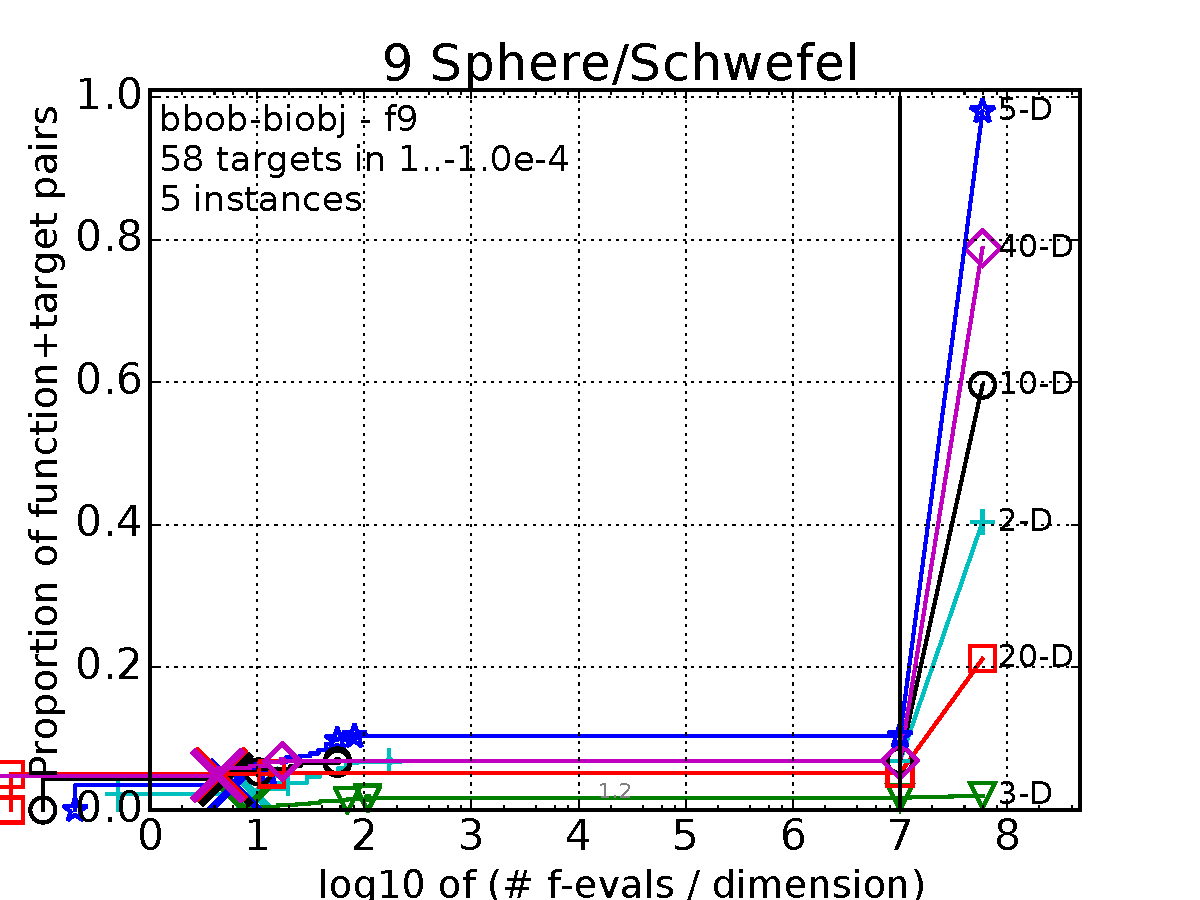
\includegraphics[width=0.25\textwidth]{pprldmany-single-functions/pprldmany_f009}&
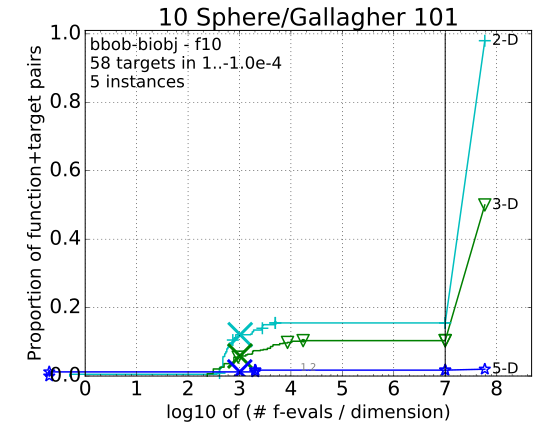
\includegraphics[width=0.25\textwidth]{pprldmany-single-functions/pprldmany_f010}&
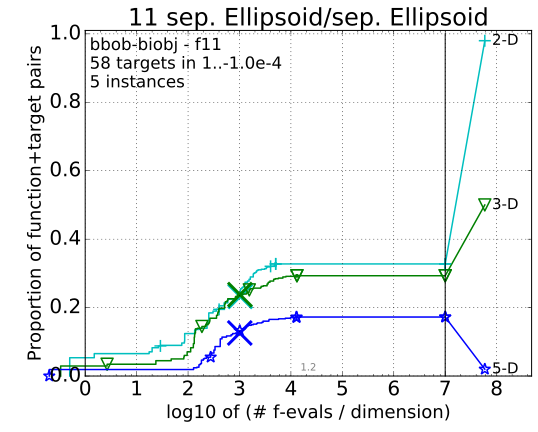
\includegraphics[width=0.25\textwidth]{pprldmany-single-functions/pprldmany_f011}&
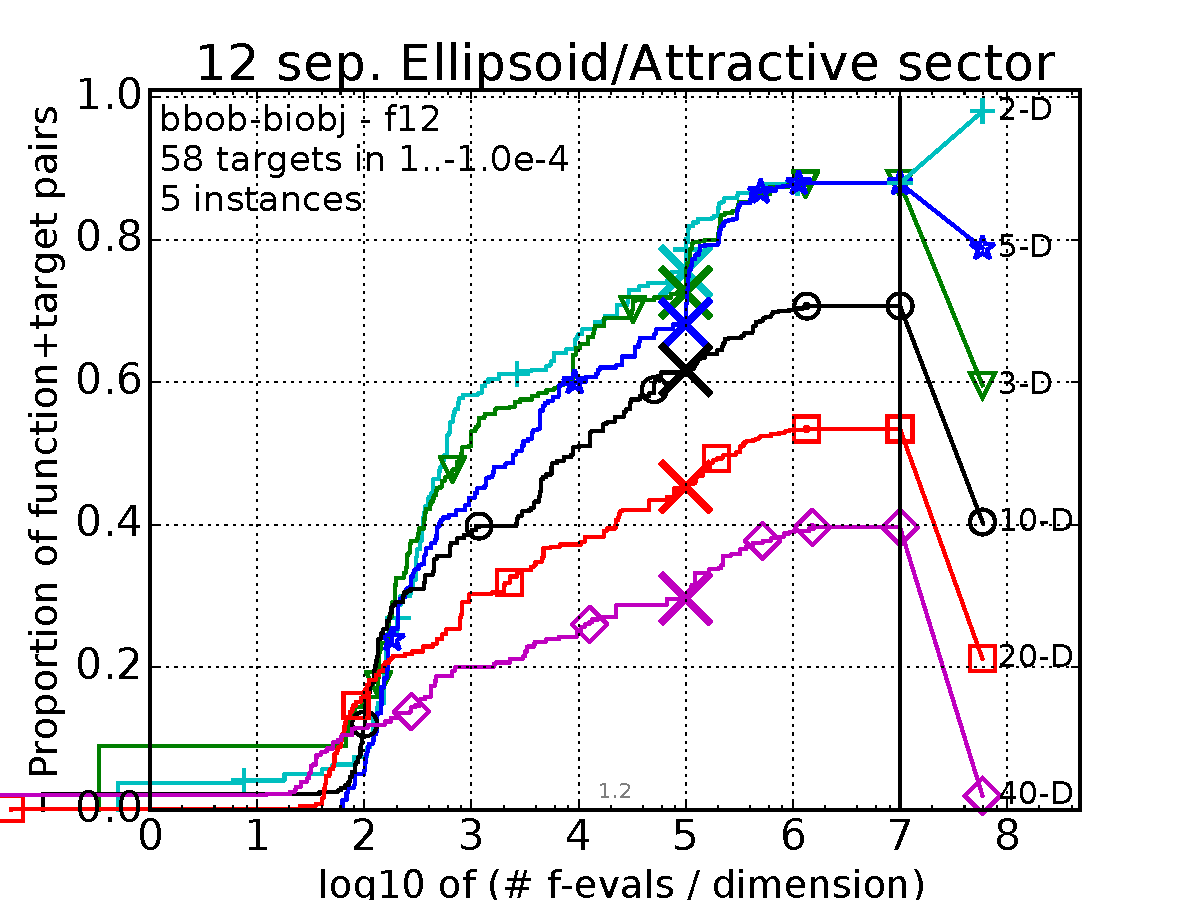
\includegraphics[width=0.25\textwidth]{pprldmany-single-functions/pprldmany_f012}\\[-1.8ex]
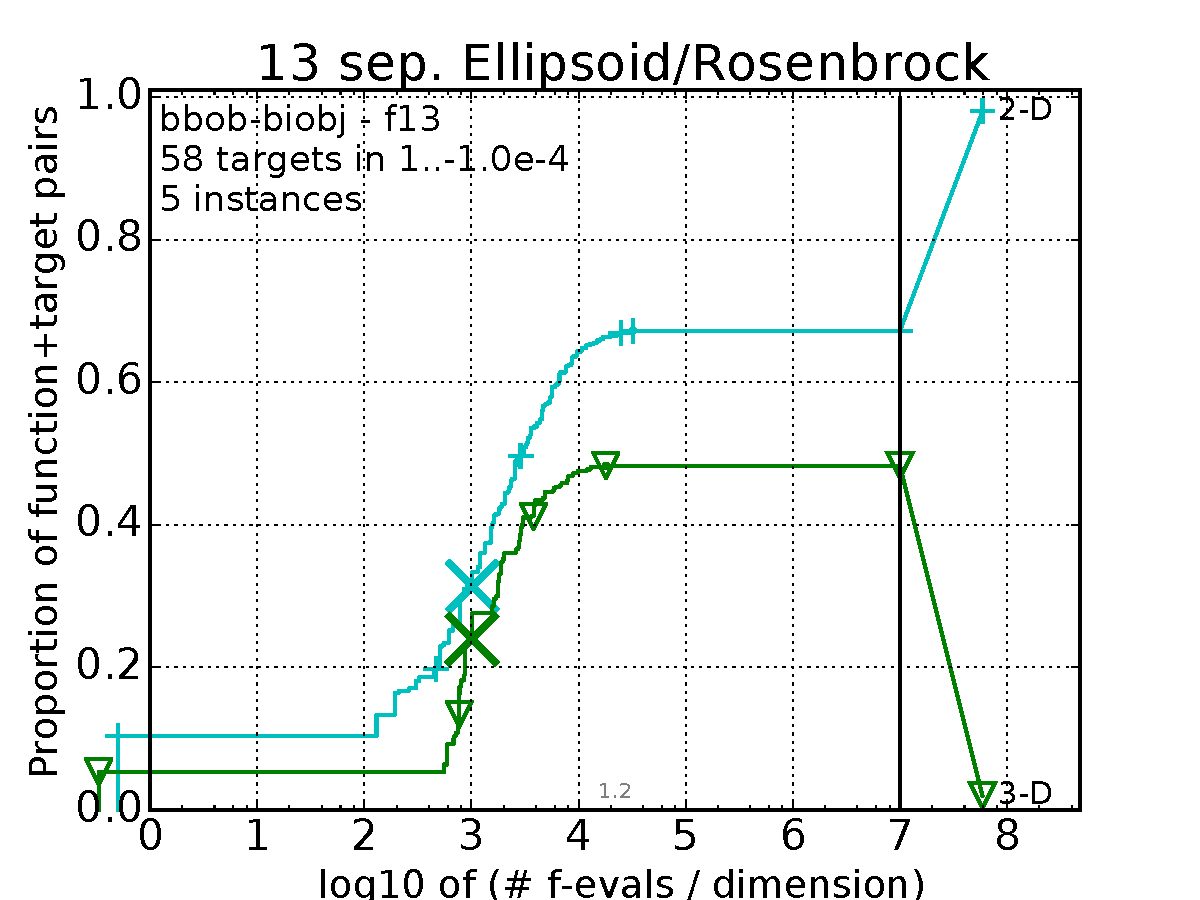
\includegraphics[width=0.25\textwidth]{pprldmany-single-functions/pprldmany_f013}&
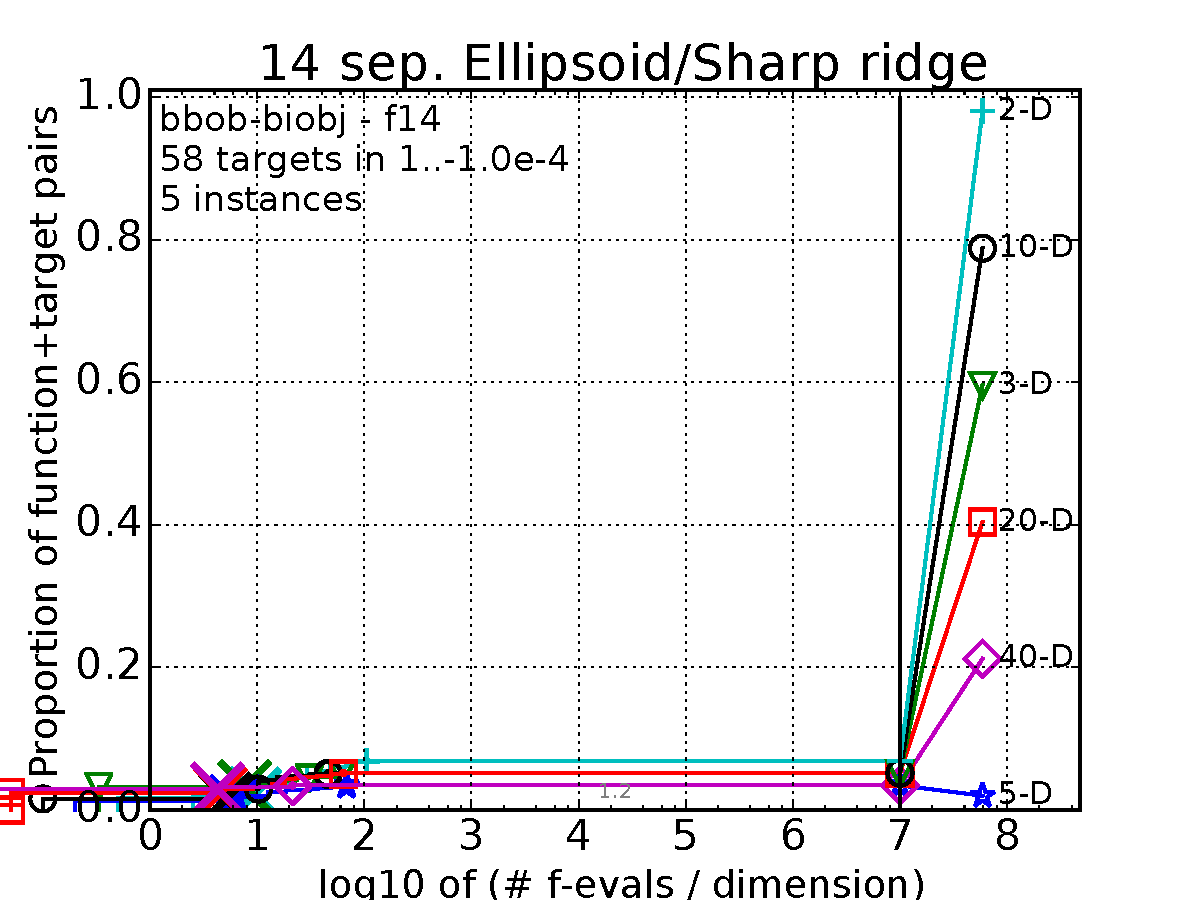
\includegraphics[width=0.25\textwidth]{pprldmany-single-functions/pprldmany_f014}&
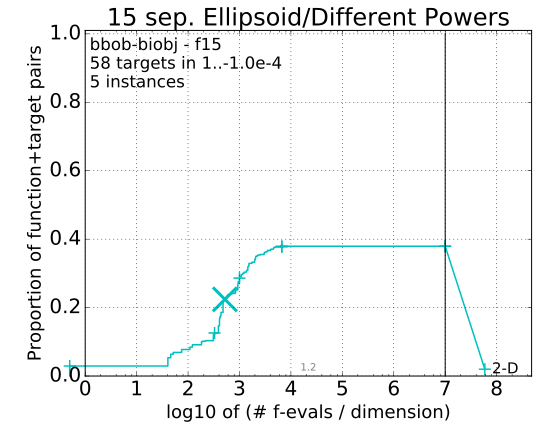
\includegraphics[width=0.25\textwidth]{pprldmany-single-functions/pprldmany_f015}&
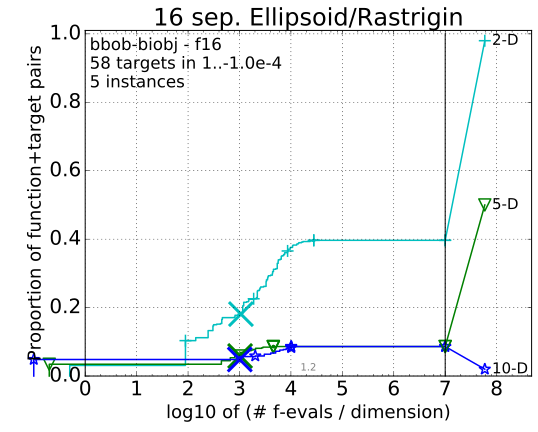
\includegraphics[width=0.25\textwidth]{pprldmany-single-functions/pprldmany_f016}\\[-1.8ex]
\end{tabular}
 \caption{\label{fig:ECDFsingleOne}
 \bbobecdfcaptionsinglefcts{}
}

\end{figure*}
\begin{figure*}
\centering
\begin{tabular}{@{\hspace*{-0.018\textwidth}}l@{\hspace*{-0.02\textwidth}}l@{\hspace*{-0.02\textwidth}}l@{\hspace*{-0.02\textwidth}}l@{\hspace*{-0.02\textwidth}}l@{\hspace*{-0.02\textwidth}}}
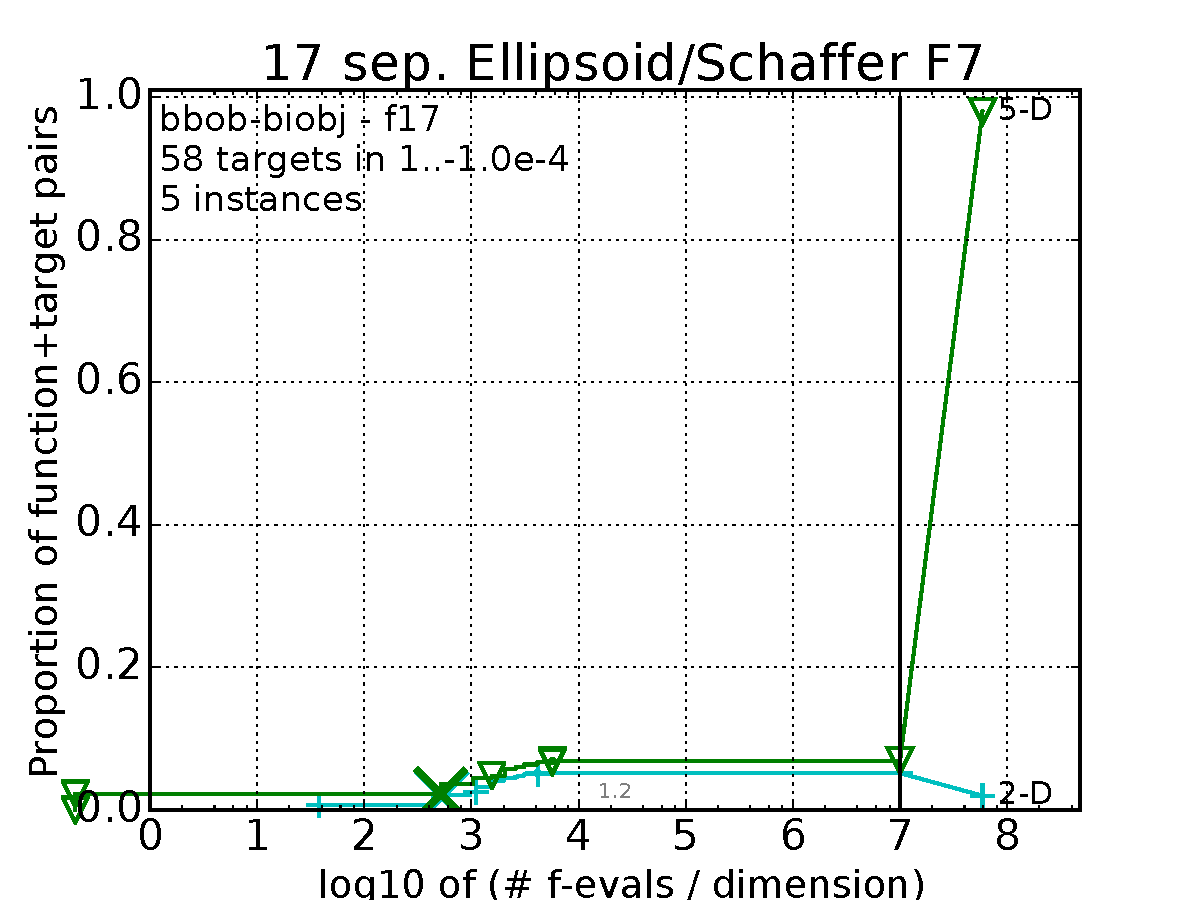
\includegraphics[width=0.25\textwidth]{pprldmany-single-functions/pprldmany_f017}&
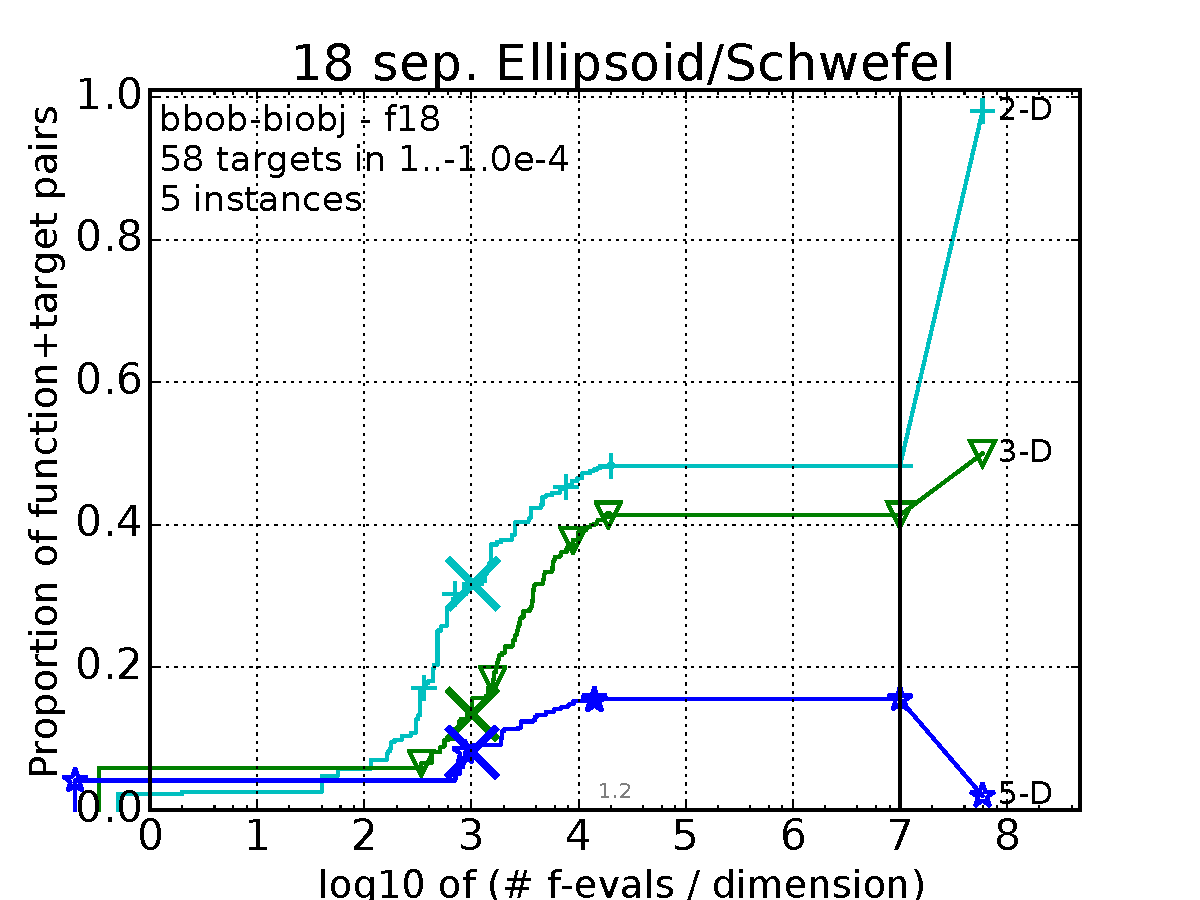
\includegraphics[width=0.25\textwidth]{pprldmany-single-functions/pprldmany_f018}&
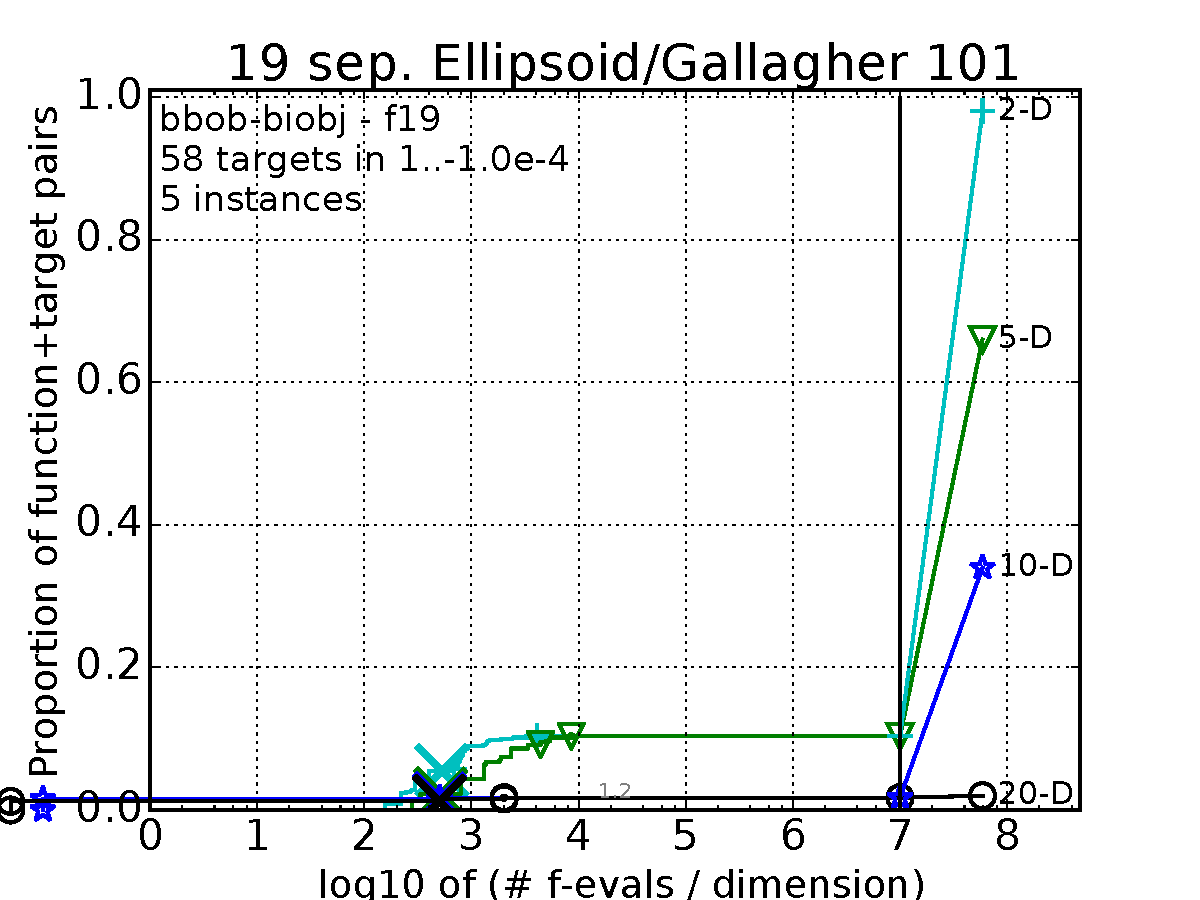
\includegraphics[width=0.25\textwidth]{pprldmany-single-functions/pprldmany_f019}&
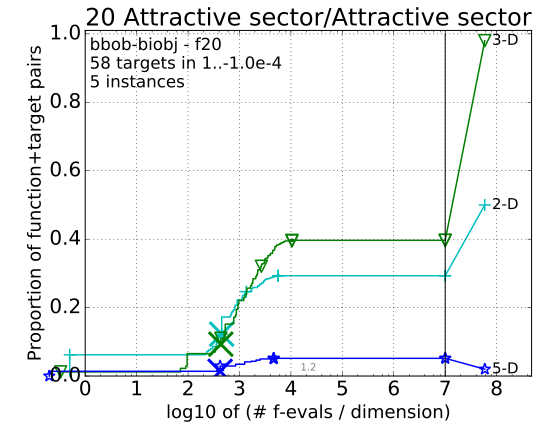
\includegraphics[width=0.25\textwidth]{pprldmany-single-functions/pprldmany_f020}\\[-1.8ex]
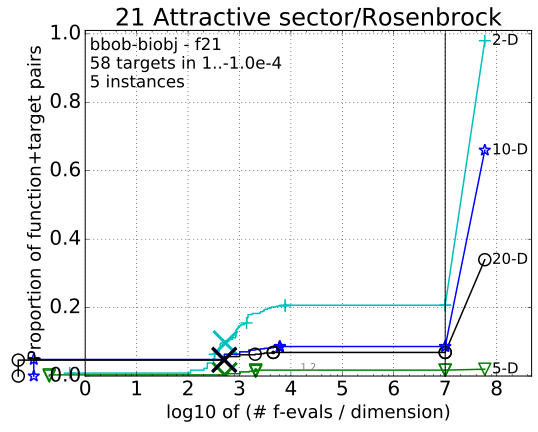
\includegraphics[width=0.25\textwidth]{pprldmany-single-functions/pprldmany_f021}&
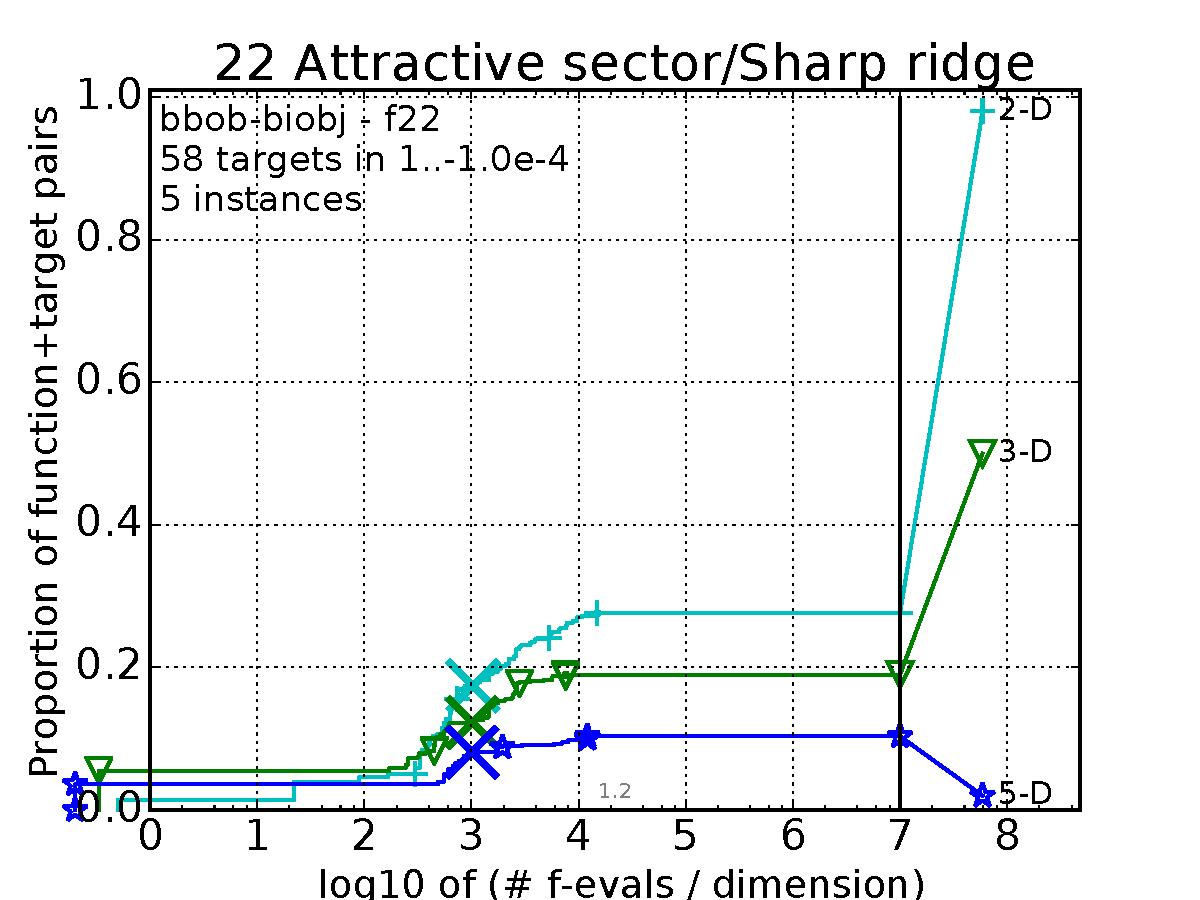
\includegraphics[width=0.25\textwidth]{pprldmany-single-functions/pprldmany_f022}&
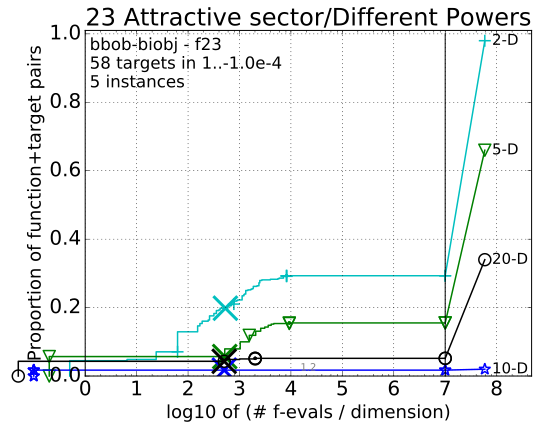
\includegraphics[width=0.25\textwidth]{pprldmany-single-functions/pprldmany_f023}&
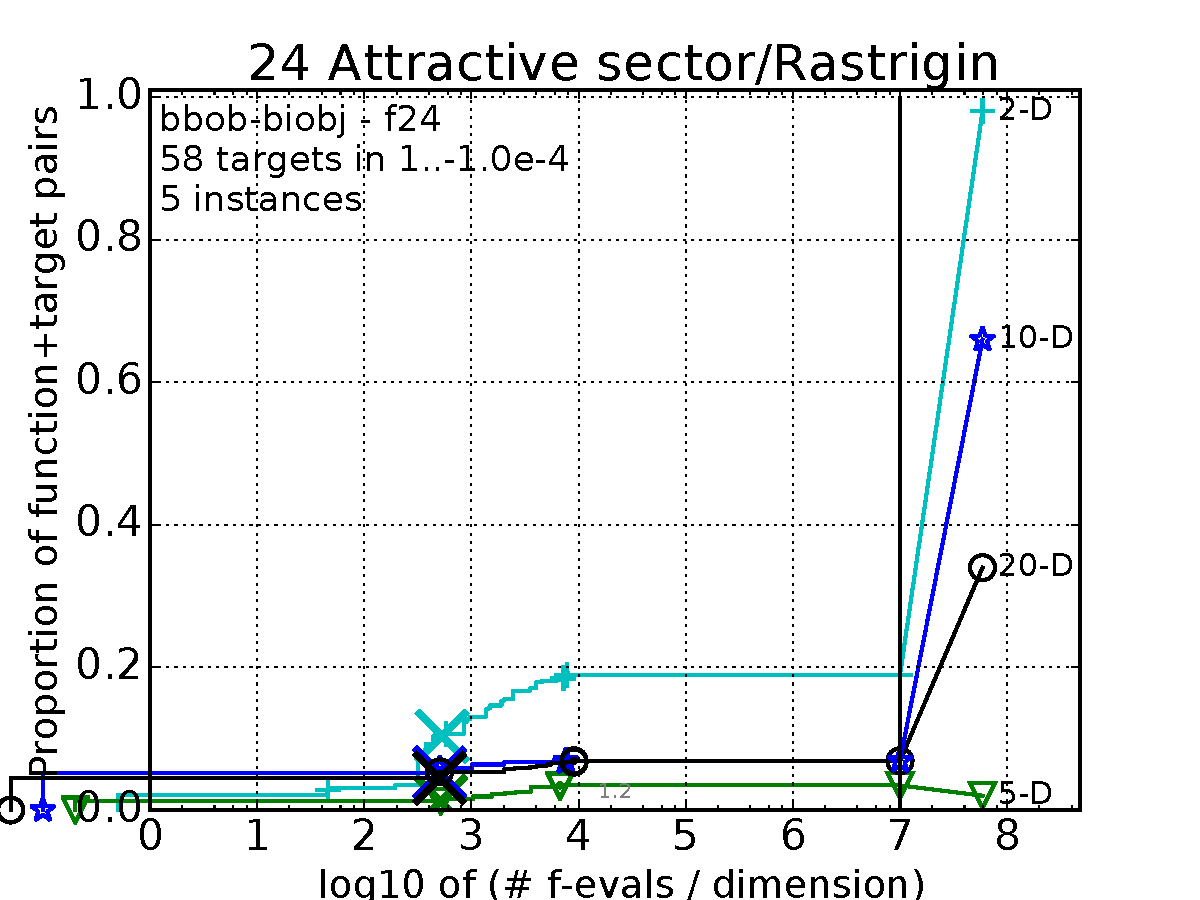
\includegraphics[width=0.25\textwidth]{pprldmany-single-functions/pprldmany_f024}\\[-1.8ex]
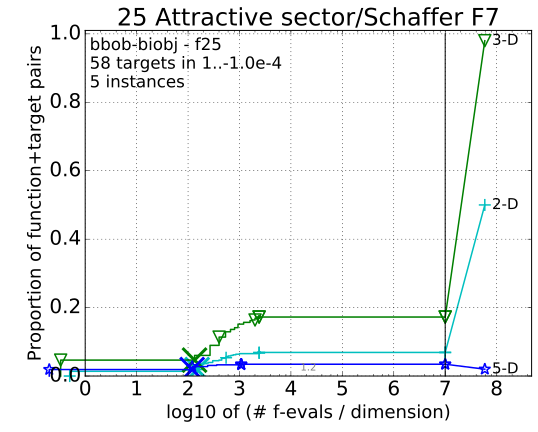
\includegraphics[width=0.25\textwidth]{pprldmany-single-functions/pprldmany_f025}&
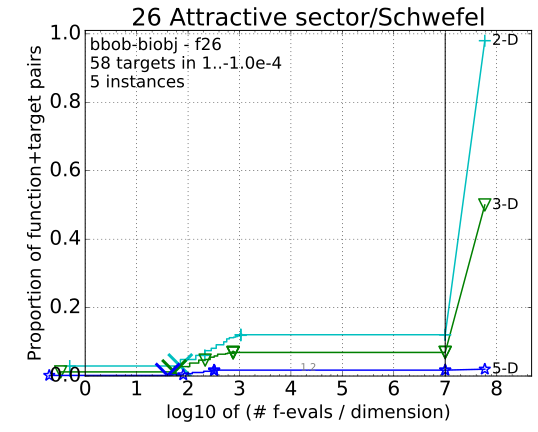
\includegraphics[width=0.25\textwidth]{pprldmany-single-functions/pprldmany_f026}&
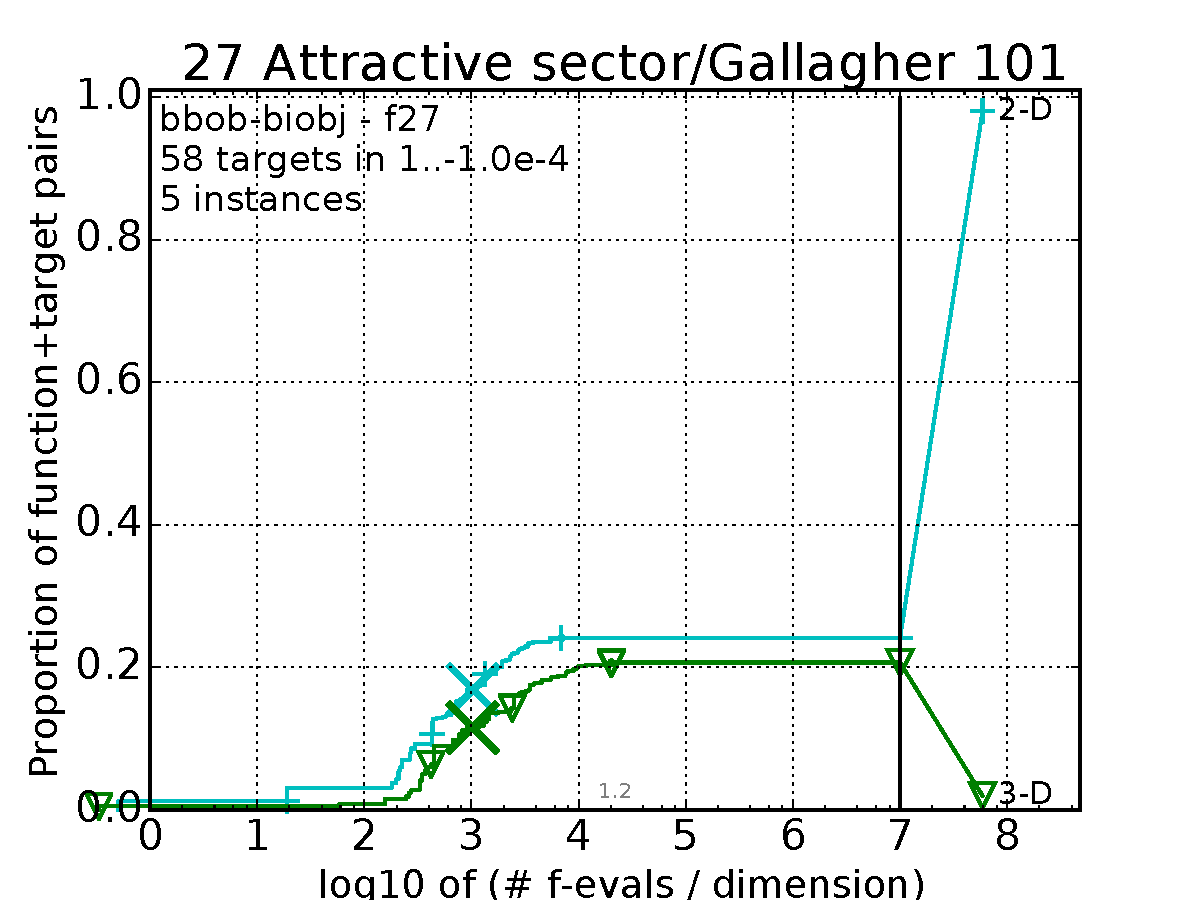
\includegraphics[width=0.25\textwidth]{pprldmany-single-functions/pprldmany_f027}&
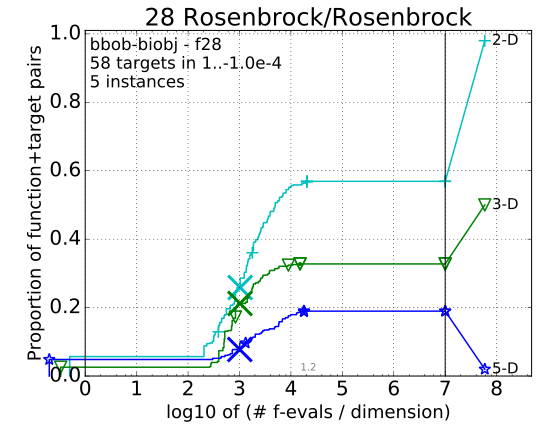
\includegraphics[width=0.25\textwidth]{pprldmany-single-functions/pprldmany_f028}\\[-1.8ex]
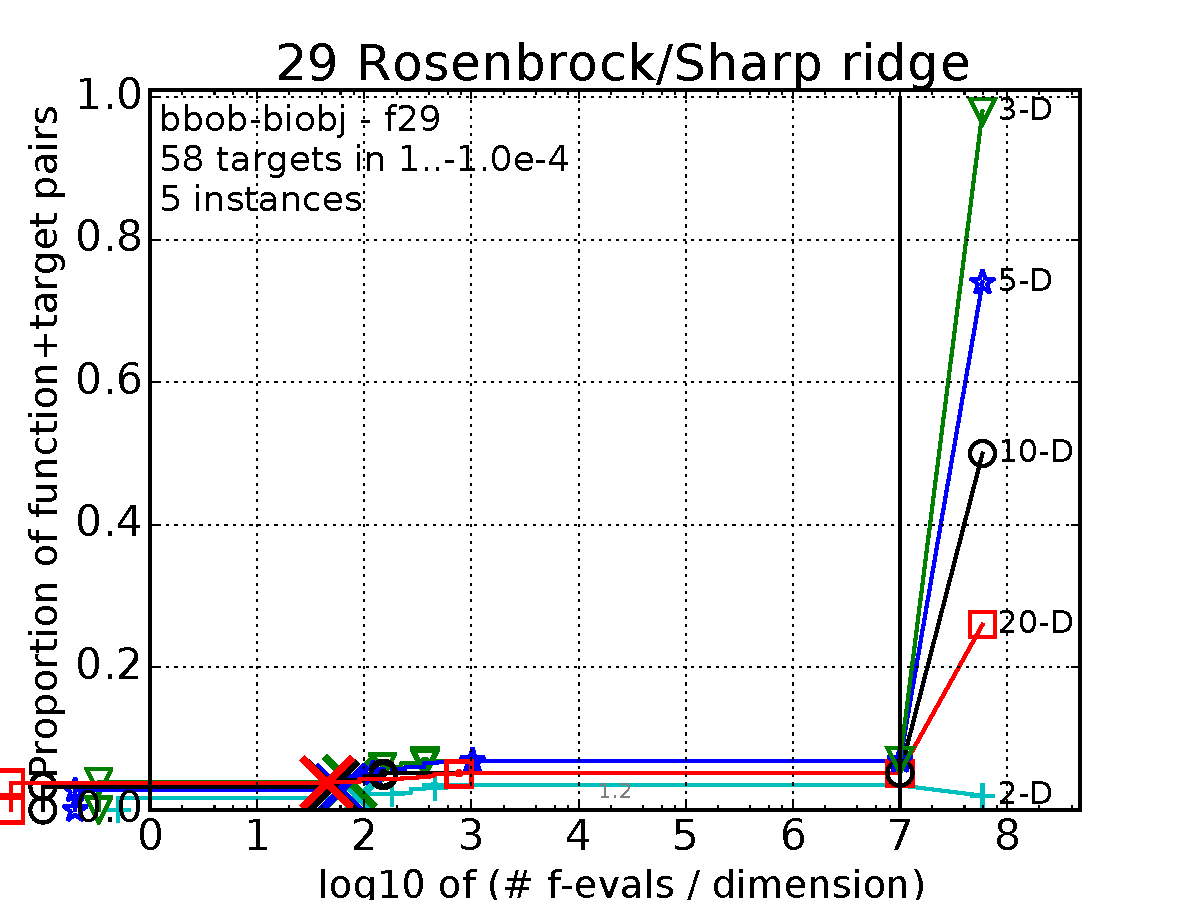
\includegraphics[width=0.25\textwidth]{pprldmany-single-functions/pprldmany_f029}&
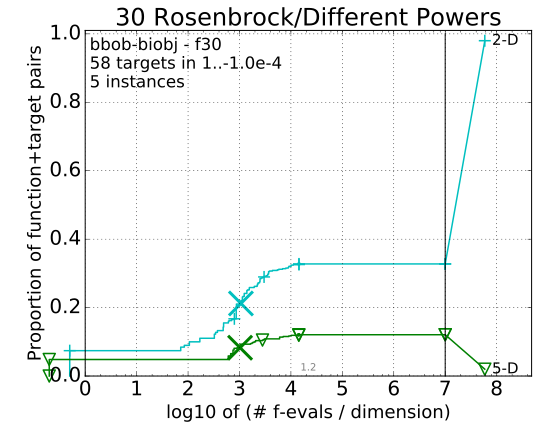
\includegraphics[width=0.25\textwidth]{pprldmany-single-functions/pprldmany_f030}&
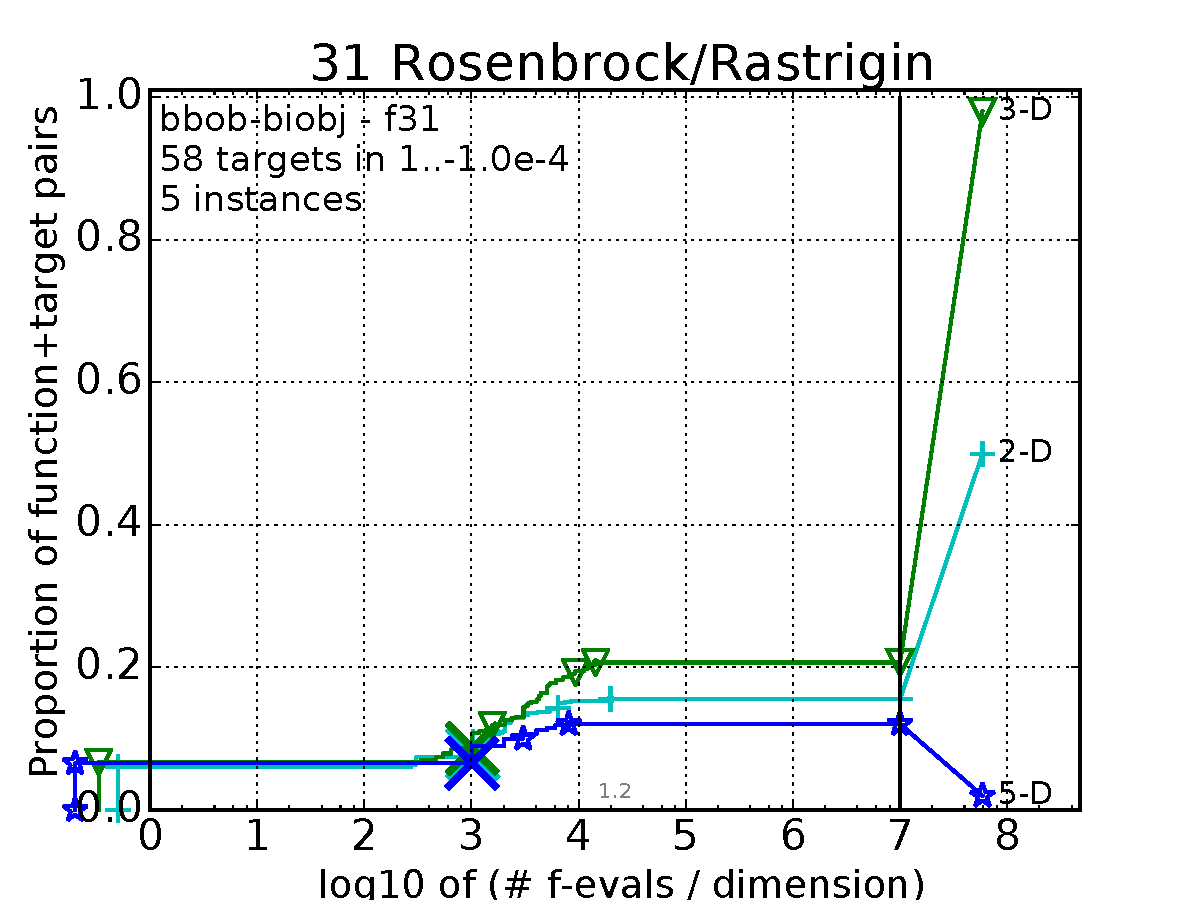
\includegraphics[width=0.25\textwidth]{pprldmany-single-functions/pprldmany_f031}&
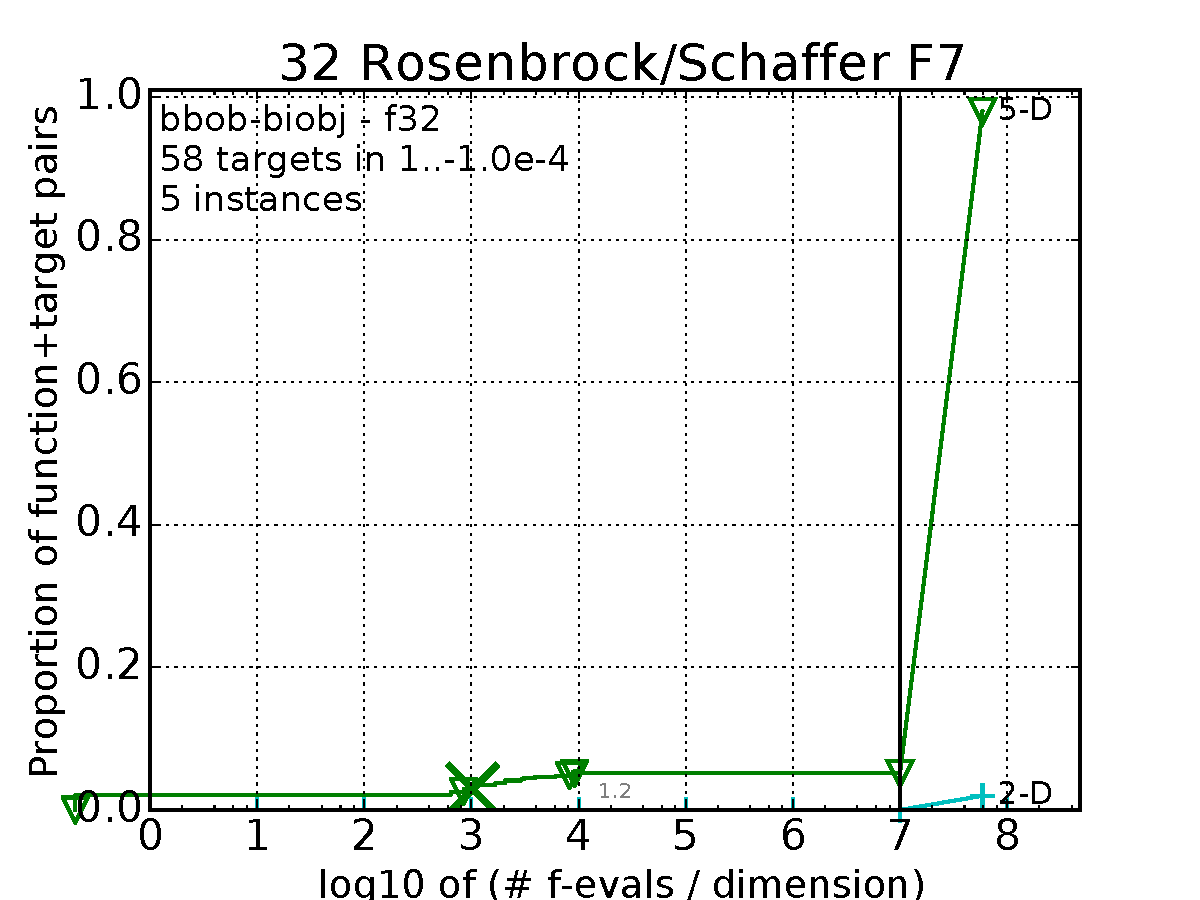
\includegraphics[width=0.25\textwidth]{pprldmany-single-functions/pprldmany_f032}\\[-1.8ex]
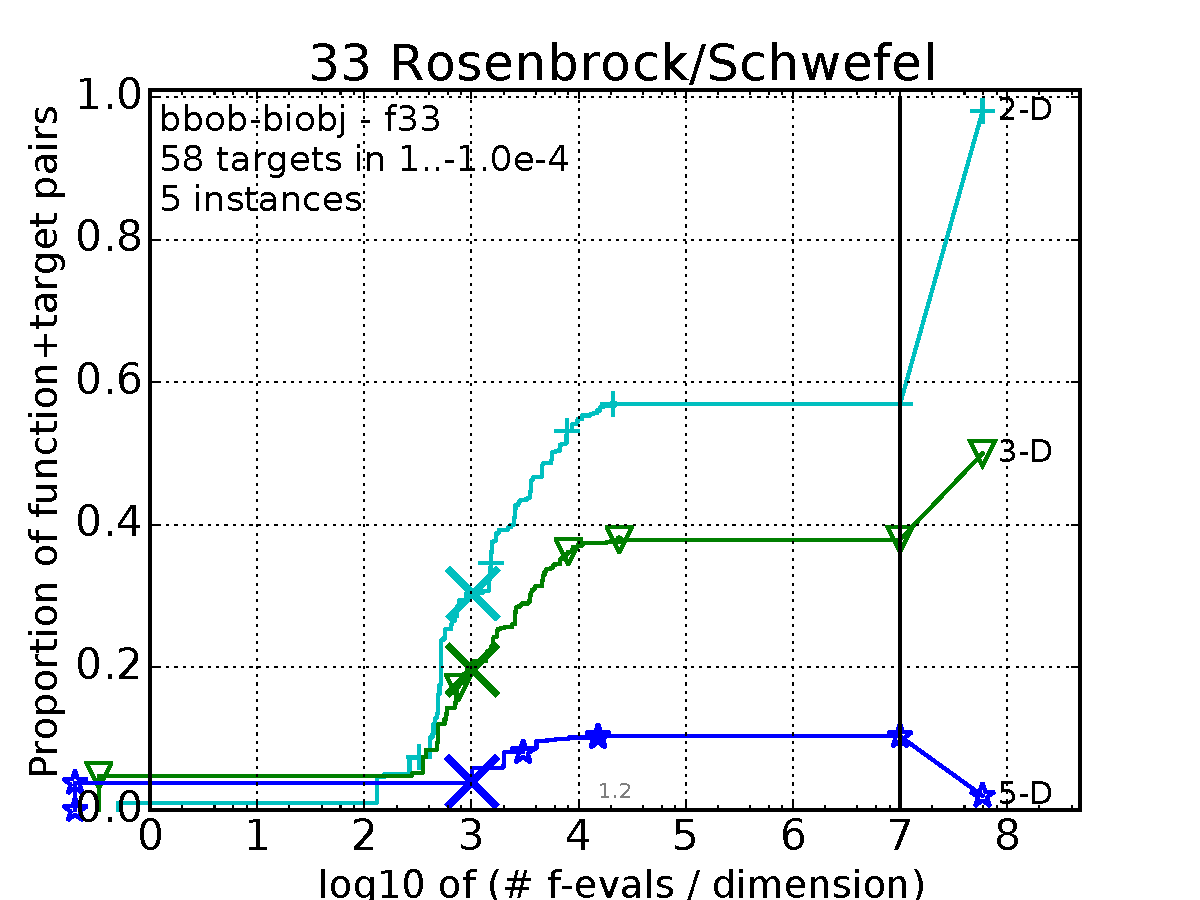
\includegraphics[width=0.25\textwidth]{pprldmany-single-functions/pprldmany_f033}&
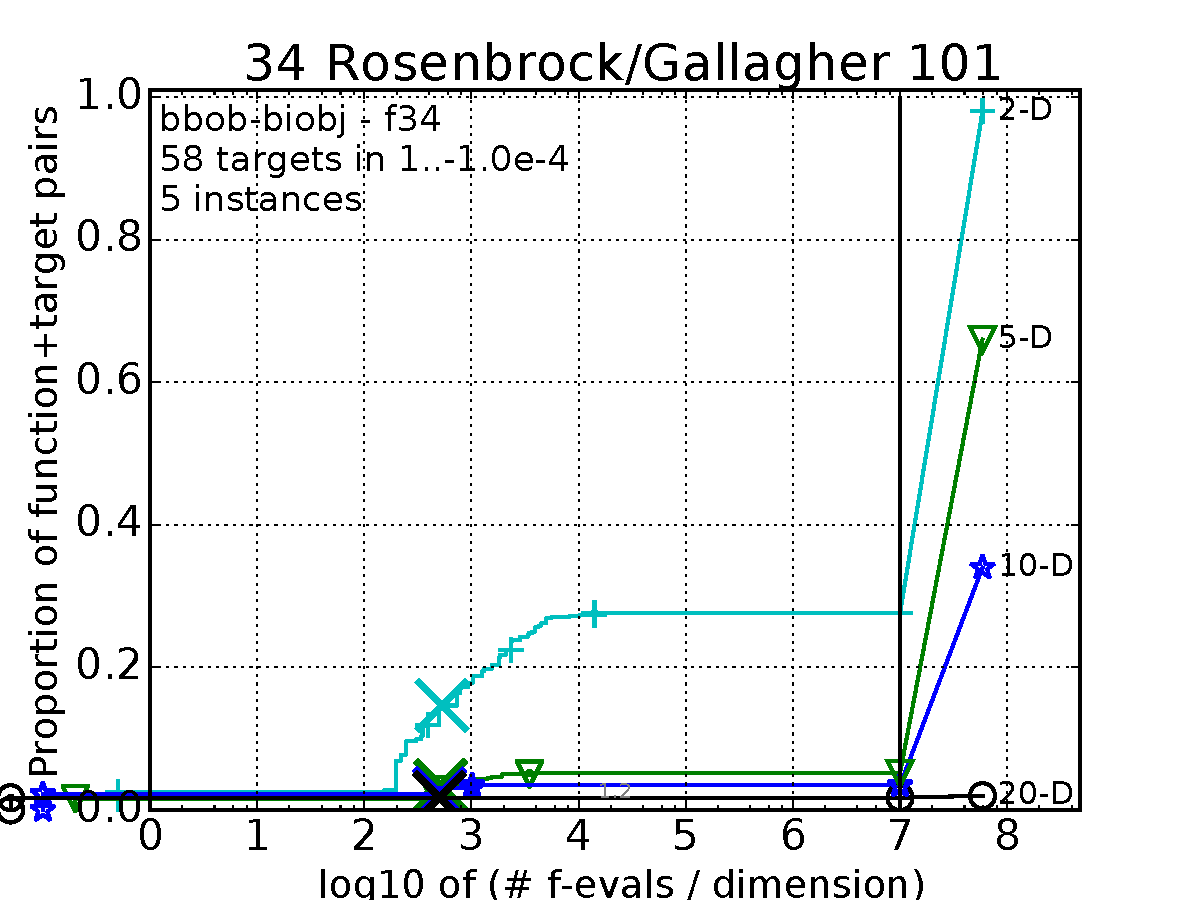
\includegraphics[width=0.25\textwidth]{pprldmany-single-functions/pprldmany_f034}&
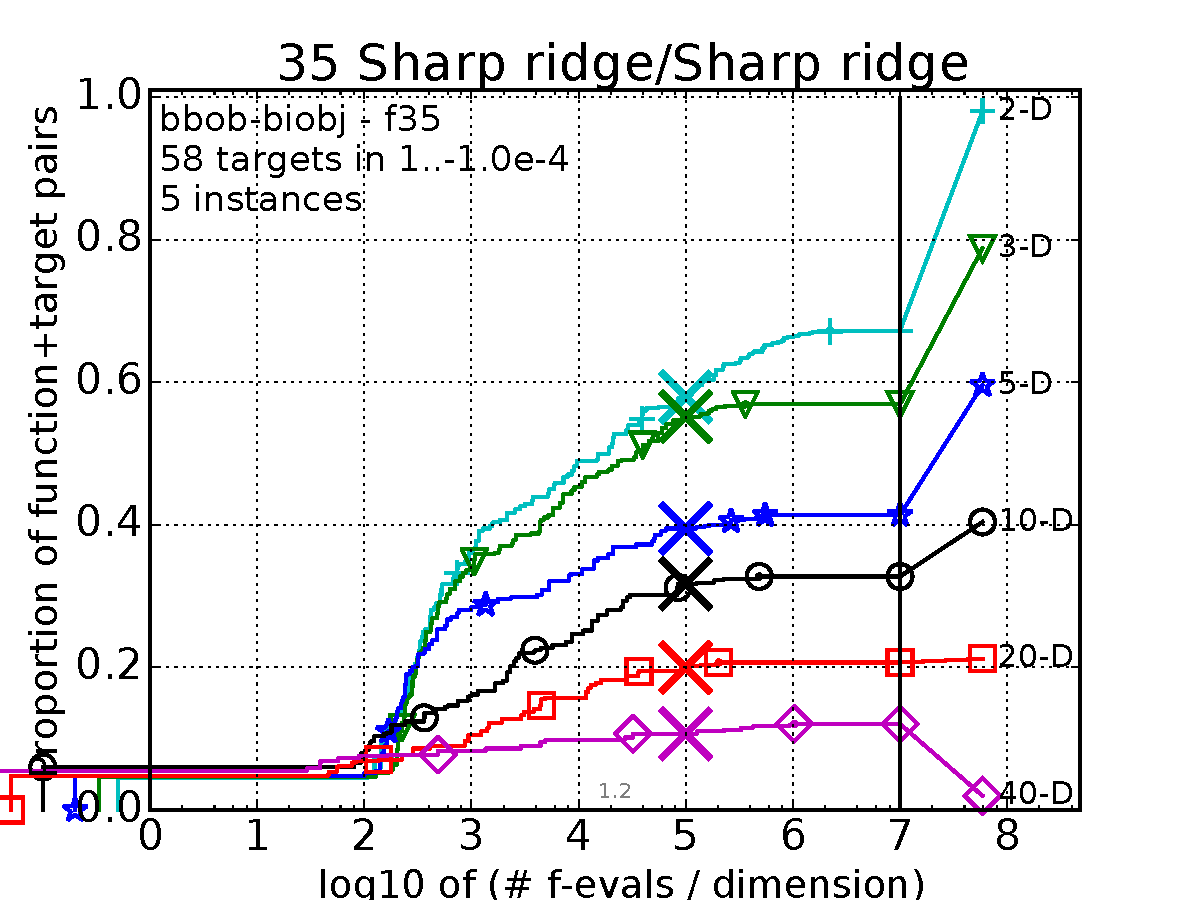
\includegraphics[width=0.25\textwidth]{pprldmany-single-functions/pprldmany_f035}&
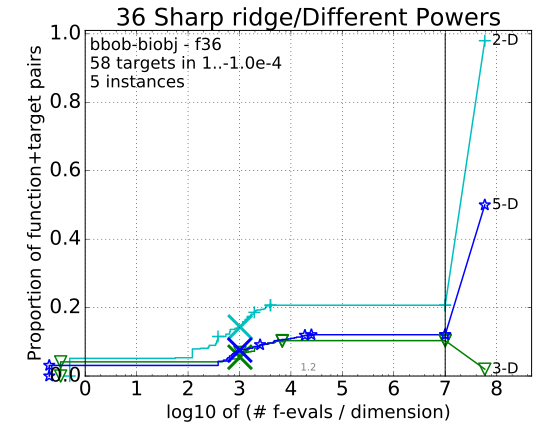
\includegraphics[width=0.25\textwidth]{pprldmany-single-functions/pprldmany_f036}\\[-1.8ex]
\end{tabular}
 \caption{\label{fig:ECDFsingleTwo}
    Empirical cumulative distribution of simulated (bootstrapped) runtimes, 
    measured in number of objective function evaluations, divided by dimension 
    (FEvals/DIM) for the targets as given in Fig.~\ref{fig:ECDFsingleOne} 
    for functions 
    $f_{17}$ to $f_{36}$
    and all dimensions.
%
% Empirical cumulative distribution function (ECDF) per dimension for all 
% targets of each function as in Fig.~\ref{fig:ECDFsingleOne} but for $f_{17}$ till $f_{36}$.
 }
\end{figure*}
\begin{figure*}
\centering
\begin{tabular}{@{\hspace*{-0.018\textwidth}}l@{\hspace*{-0.02\textwidth}}l@{\hspace*{-0.02\textwidth}}l@{\hspace*{-0.02\textwidth}}l@{\hspace*{-0.02\textwidth}}l@{\hspace*{-0.02\textwidth}}}
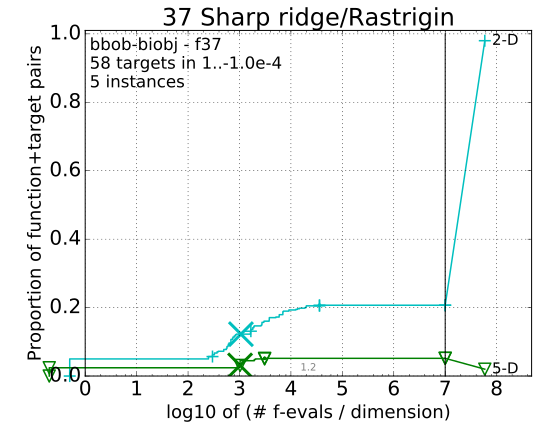
\includegraphics[width=0.25\textwidth]{pprldmany-single-functions/pprldmany_f037}&
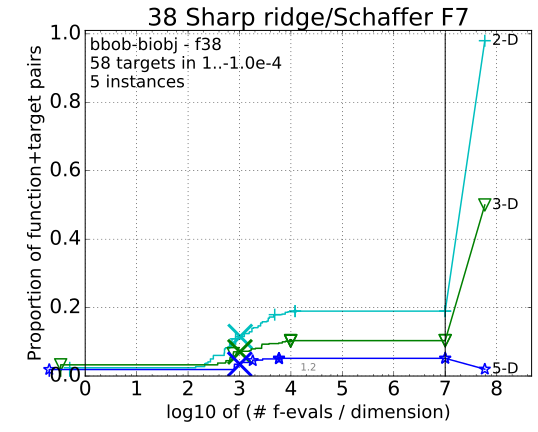
\includegraphics[width=0.25\textwidth]{pprldmany-single-functions/pprldmany_f038}&
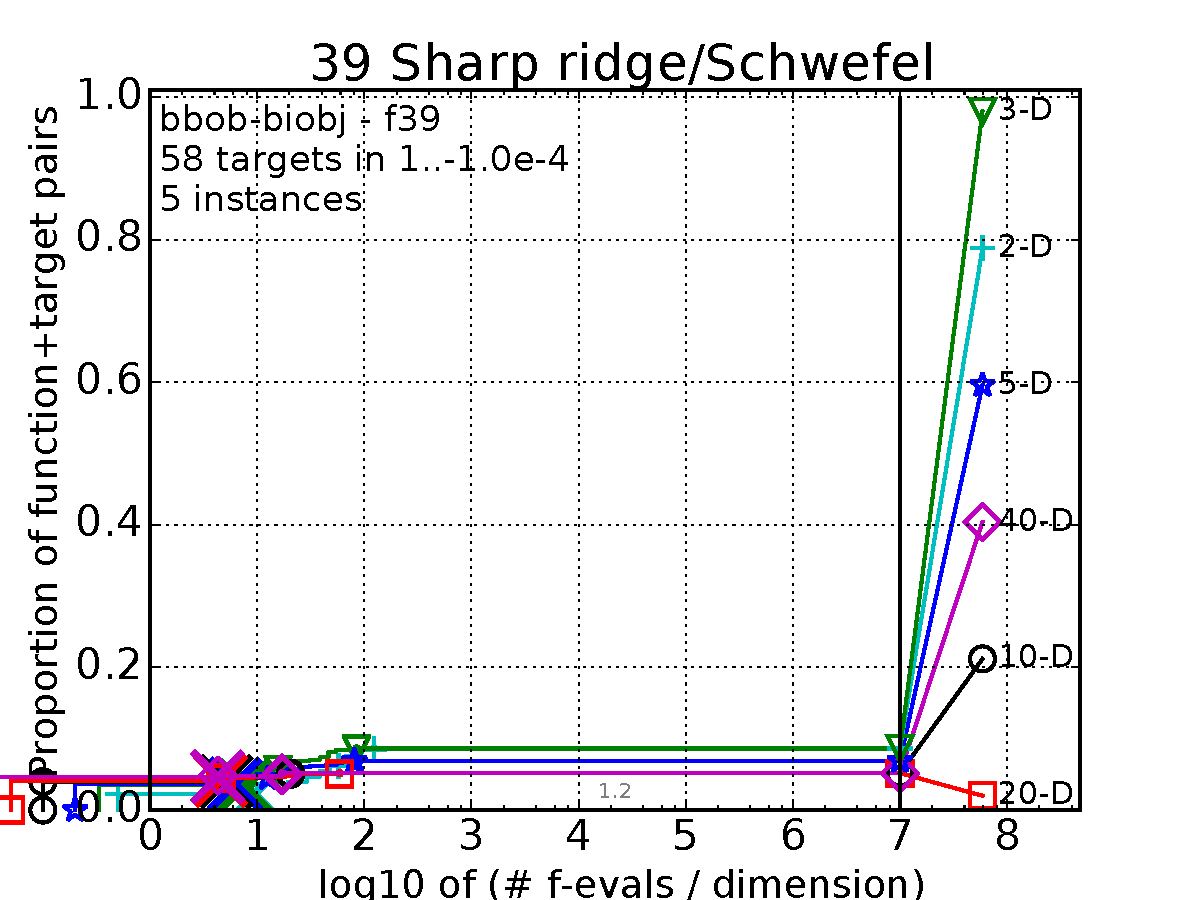
\includegraphics[width=0.25\textwidth]{pprldmany-single-functions/pprldmany_f039}&
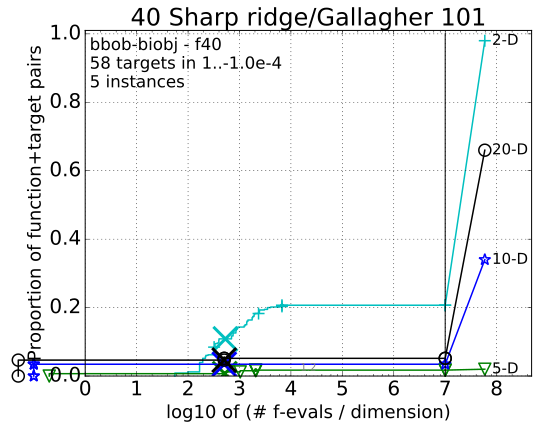
\includegraphics[width=0.25\textwidth]{pprldmany-single-functions/pprldmany_f040}\\[-1.8ex]
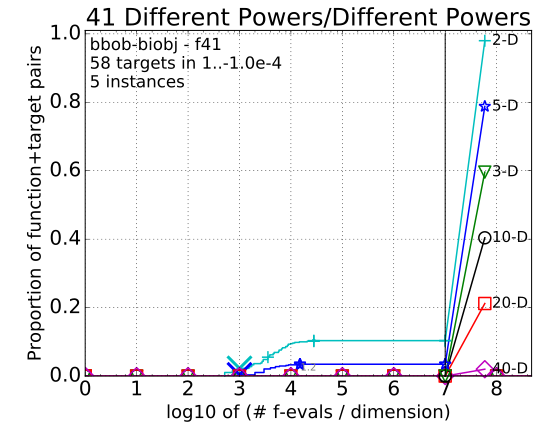
\includegraphics[width=0.25\textwidth]{pprldmany-single-functions/pprldmany_f041}&
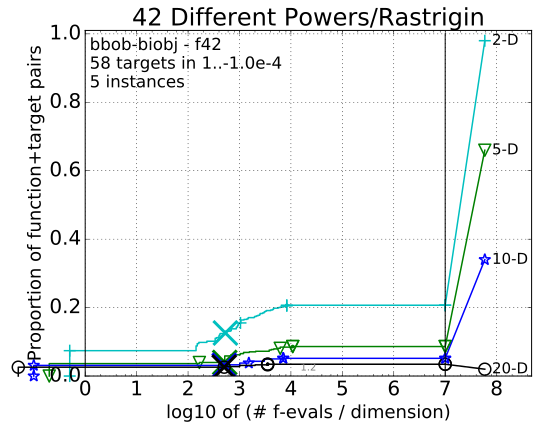
\includegraphics[width=0.25\textwidth]{pprldmany-single-functions/pprldmany_f042}&
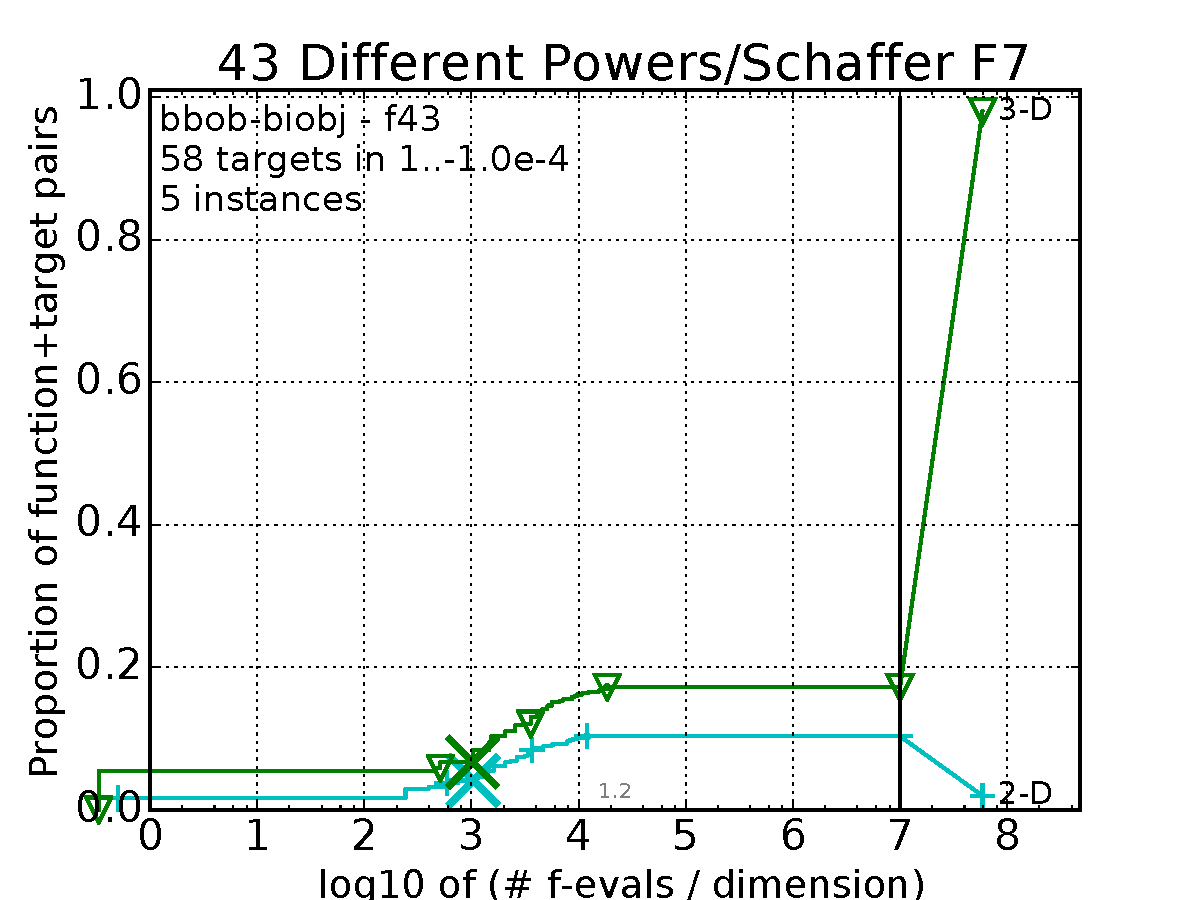
\includegraphics[width=0.25\textwidth]{pprldmany-single-functions/pprldmany_f043}&
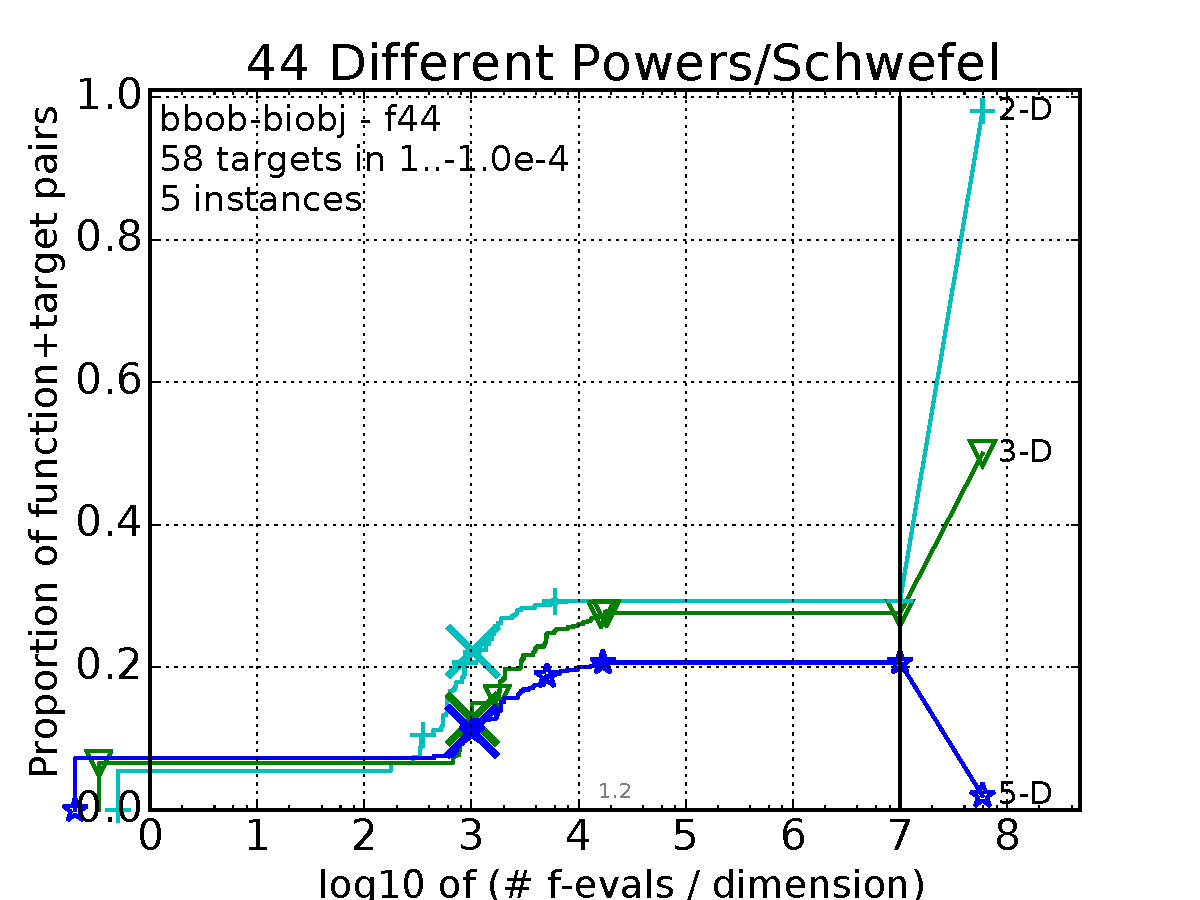
\includegraphics[width=0.25\textwidth]{pprldmany-single-functions/pprldmany_f044}\\[-1.8ex]
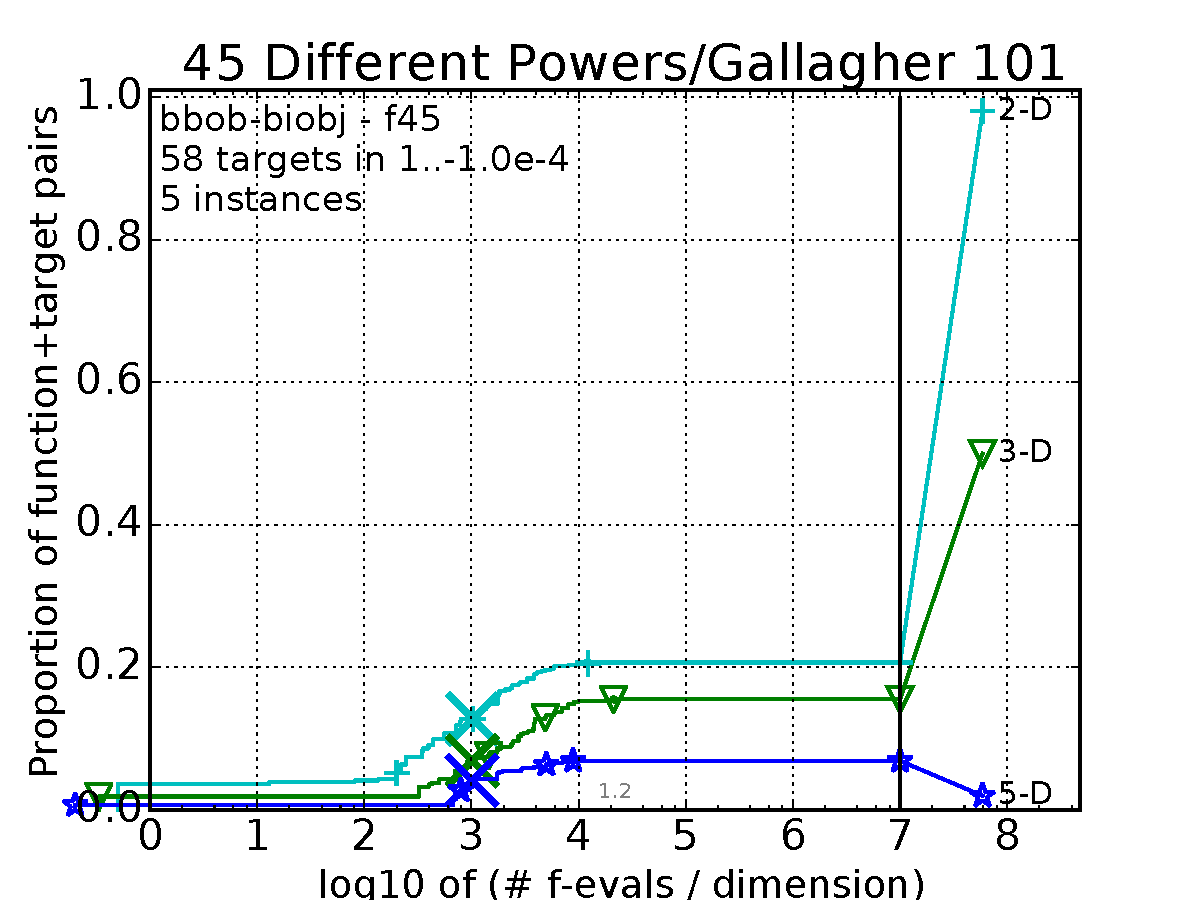
\includegraphics[width=0.25\textwidth]{pprldmany-single-functions/pprldmany_f045}&
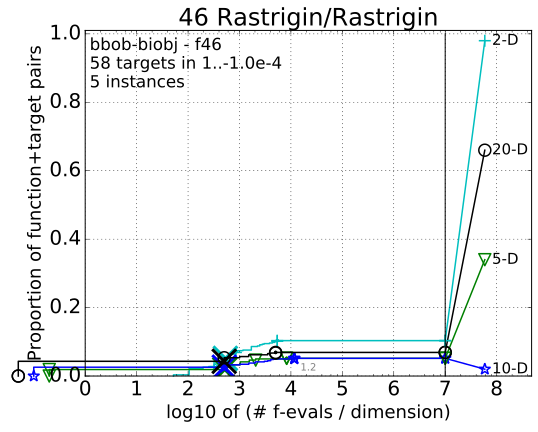
\includegraphics[width=0.25\textwidth]{pprldmany-single-functions/pprldmany_f046}&
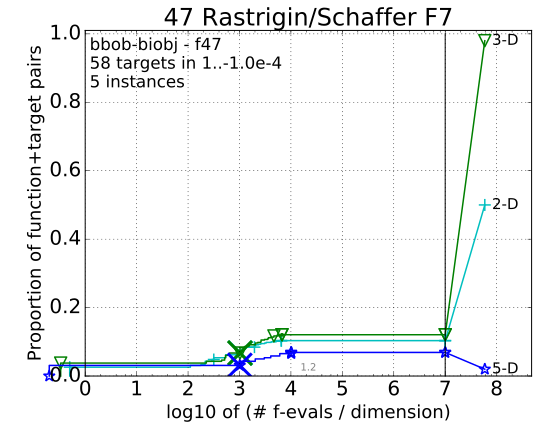
\includegraphics[width=0.25\textwidth]{pprldmany-single-functions/pprldmany_f047}&
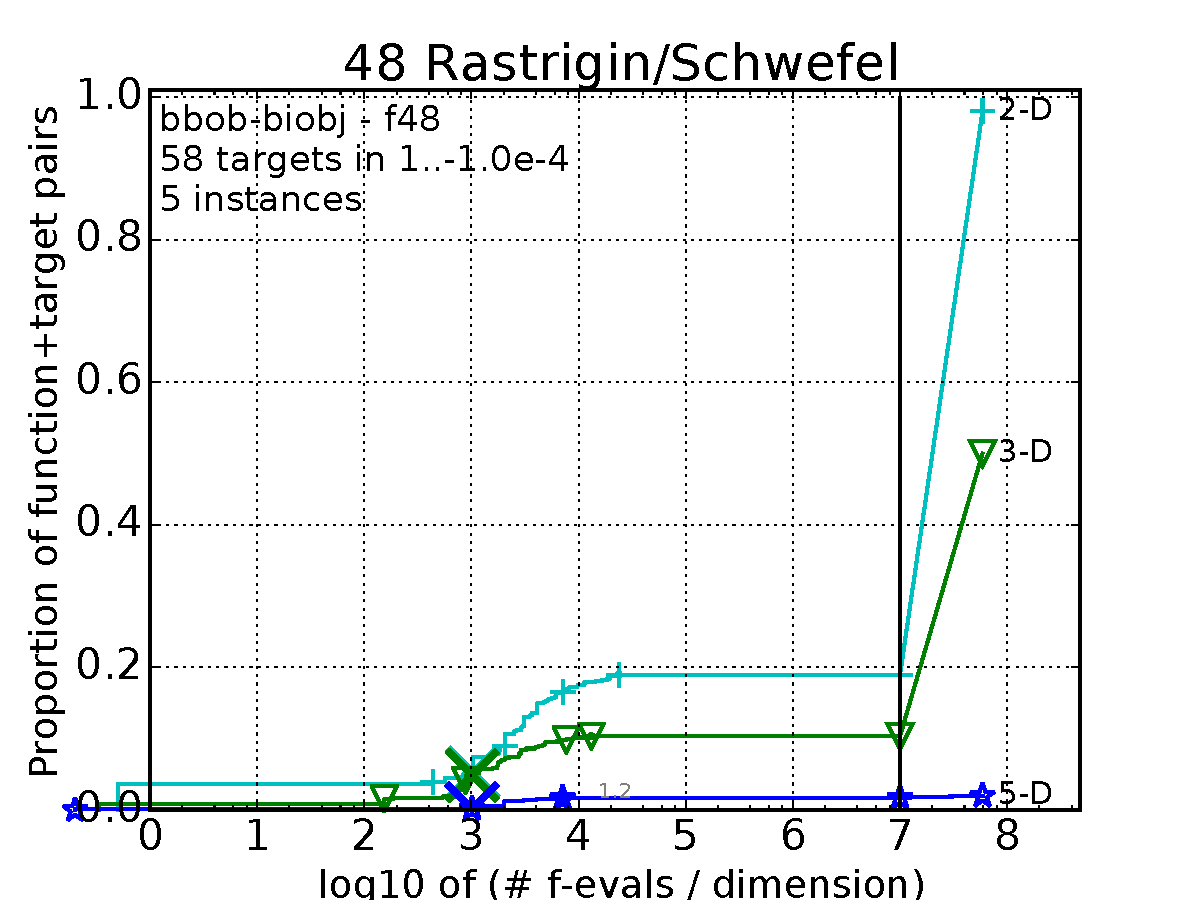
\includegraphics[width=0.25\textwidth]{pprldmany-single-functions/pprldmany_f048}\\[-1.8ex]
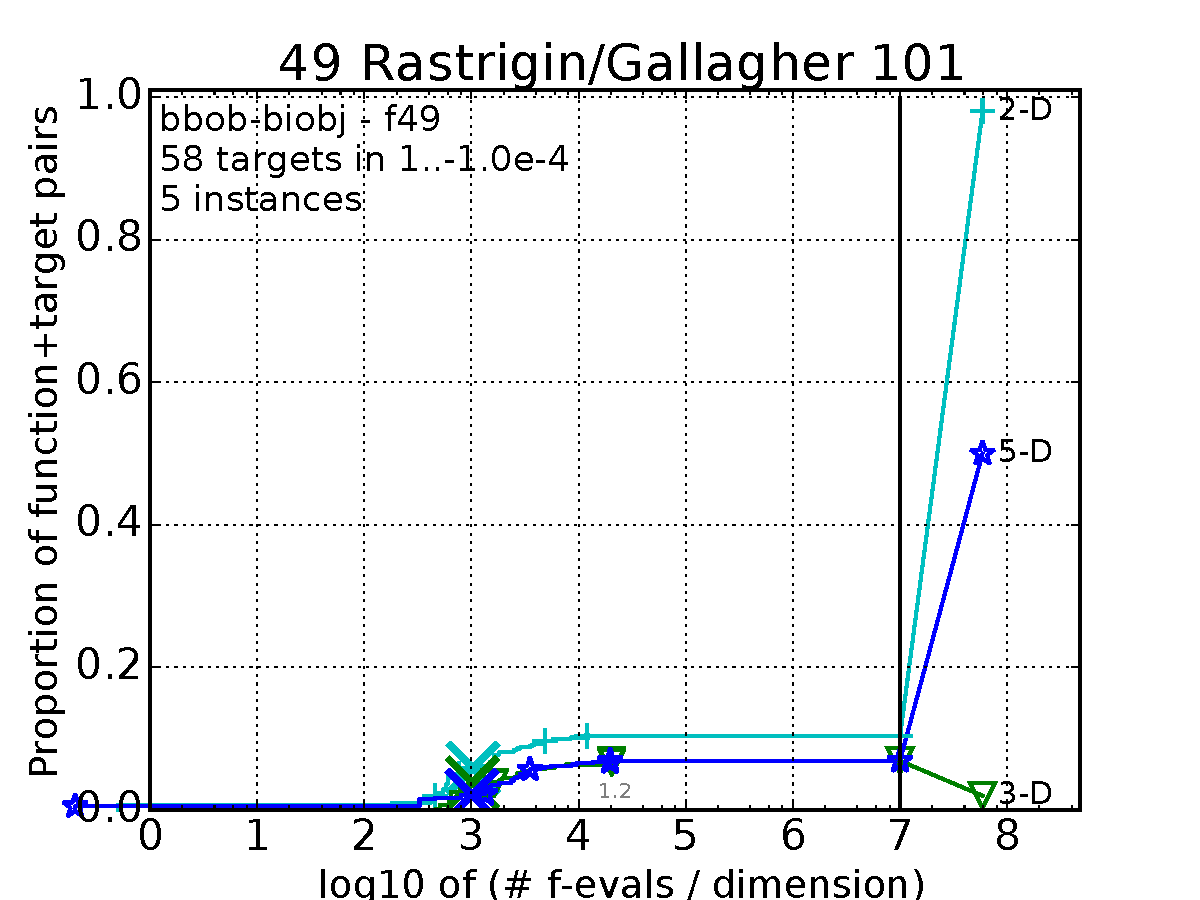
\includegraphics[width=0.25\textwidth]{pprldmany-single-functions/pprldmany_f049}&
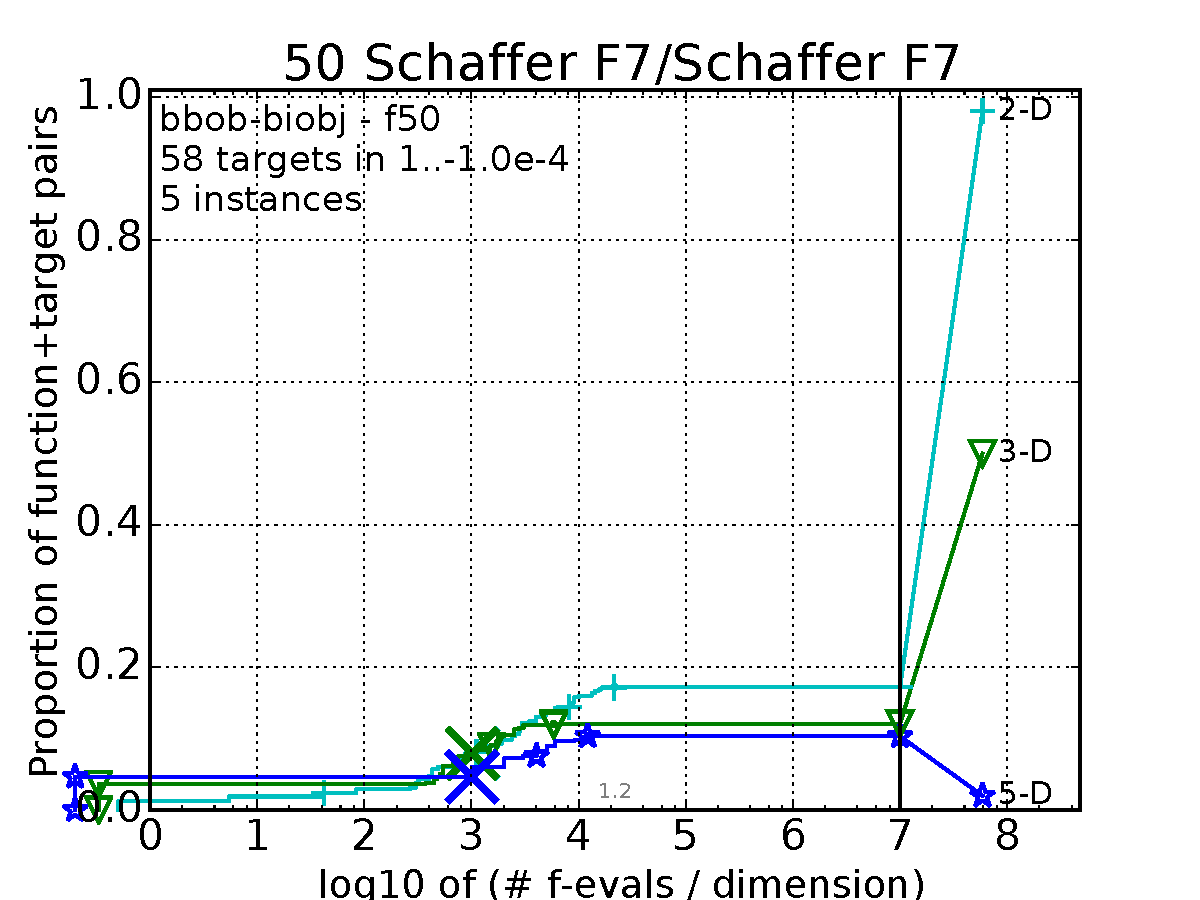
\includegraphics[width=0.25\textwidth]{pprldmany-single-functions/pprldmany_f050}&
\includegraphics[width=0.25\textwidth]{pprldmany-single-functions/pprldmany_f051}&
\includegraphics[width=0.25\textwidth]{pprldmany-single-functions/pprldmany_f052}
\end{tabular}
\begin{tabular}{@{\hspace*{-0.018\textwidth}}l@{\hspace*{-0.02\textwidth}}l@{\hspace*{-0.02\textwidth}}l@{\hspace*{-0.02\textwidth}}l@{\hspace*{-0.02\textwidth}}}
\includegraphics[width=0.25\textwidth]{pprldmany-single-functions/pprldmany_f053}&
\includegraphics[width=0.25\textwidth]{pprldmany-single-functions/pprldmany_f054}&
\includegraphics[width=0.25\textwidth]{pprldmany-single-functions/pprldmany_f055}\\[-1.8ex]
\end{tabular}
 \caption{\label{fig:ECDFsingleThree}
    Empirical cumulative distribution of simulated (bootstrapped) runtimes, 
    measured in number of objective function evaluations, divided by dimension 
    (FEvals/DIM) for the targets as given in Fig.~\ref{fig:ECDFsingleOne} 
    for functions 
    $f_{37}$ to $f_{55}$
    and all dimensions. 
% Empirical cumulative distribution function (ECDF) per dimension for all targets of each function as in Fig.~\ref{fig:ECDFsingleOne} but for $f_{37}$ till $f_{55}$.
 }
\end{figure*}



%%%%%%%%%%%%%%%%%%%%%%%%%%%%%%%%%%%%%%%%%%%%%%%%%%%%%%%%%%%%%%%%%%%%%%%%%%%%%%%
%%%%%%%%%%%%%%%%%%%%%%%%%%%%%%%%%%%%%%%%%%%%%%%%%%%%%%%%%%%%%%%%%%%%%%%%%%%%%%%

% Empirical cumulative distribution functions (ECDFs) per function group.

%%%%%%%%%%%%%%%%%%%%%%%%%%%%%%%%%%%%%%%%%%%%%%%%%%%%%%%%%%%%%%%%%%%%%%%%%%%%%%%

\newcommand{\rot}[2][2.5]{
  \hspace*{-3.5\baselineskip}%
  \begin{rotate}{90}\hspace{#1em}#2
  \end{rotate}}
\begin{figure*}
\begin{tabular}{c@{\hspace*{-0.02\textwidth}}c@{\hspace*{-0.02\textwidth}}c@{\hspace*{-0.02\textwidth}}c}
separable-separable & separable-moderate & separable-ill-cond. & separable-multimodal\\
\includegraphics[width=0.268\textwidth,trim=0 0 0 13mm, clip]{pprldmany-single-functions/pprldmany_1-separable_1-separable} &
\includegraphics[width=0.268\textwidth,trim=0 0 0 13mm, clip]{pprldmany-single-functions/pprldmany_1-separable_2-moderate} &
\includegraphics[width=0.268\textwidth,trim=0 0 0 13mm, clip]{pprldmany-single-functions/pprldmany_1-separable_3-ill-conditioned} &
\includegraphics[width=0.268\textwidth,trim=0 0 0 13mm, clip]{pprldmany-single-functions/pprldmany_1-separable_4-multi-modal}\\
separable-weakstructure & moderate-moderate & moderate-ill-cond. & moderate-multimodal\\
\includegraphics[width=0.268\textwidth,trim=0 0 0 13mm, clip]{pprldmany-single-functions/pprldmany_1-separable_5-weakly-structured} &
\includegraphics[width=0.268\textwidth,trim=0 0 0 13mm, clip]{pprldmany-single-functions/pprldmany_2-moderate_2-moderate} &
\includegraphics[width=0.268\textwidth,trim=0 0 0 13mm, clip]{pprldmany-single-functions/pprldmany_2-moderate_3-ill-conditioned} &
\includegraphics[width=0.268\textwidth,trim=0 0 0 13mm, clip]{pprldmany-single-functions/pprldmany_2-moderate_4-multi-modal}\\
moderate-weakstructure & ill-cond.-ill-cond. & ill-cond.-multimodal & ill-cond.-weakstructure\\
\includegraphics[width=0.268\textwidth,trim=0 0 0 13mm, clip]{pprldmany-single-functions/pprldmany_2-moderate_5-weakly-structured} &
\includegraphics[width=0.268\textwidth,trim=0 0 0 13mm, clip]{pprldmany-single-functions/pprldmany_3-ill-conditioned_3-ill-conditioned} &
\includegraphics[width=0.268\textwidth,trim=0 0 0 13mm, clip]{pprldmany-single-functions/pprldmany_3-ill-conditioned_4-multi-modal} &
\includegraphics[width=0.268\textwidth,trim=0 0 0 13mm, clip]{pprldmany-single-functions/pprldmany_3-ill-conditioned_5-weakly-structured} \\
multimodal-multimodal & multimodal-weakstructure & weakstructure-weakstructure & all 55 functions\\
\includegraphics[width=0.268\textwidth,trim=0 0 0 13mm, clip]{pprldmany-single-functions/pprldmany_4-multi-modal_4-multi-modal} &
\includegraphics[width=0.268\textwidth,trim=0 0 0 13mm, clip]{pprldmany-single-functions/pprldmany_4-multi-modal_5-weakly-structured} &
\includegraphics[width=0.268\textwidth,trim=0 0 0 13mm, clip]{pprldmany-single-functions/pprldmany_5-weakly-structured_5-weakly-structured} &
\includegraphics[width=0.268\textwidth,trim=0 0 0 13mm, clip]{pprldmany-single-functions/pprldmany}
\vspace*{-0.5ex}
\end{tabular}
 \caption{\label{fig:ECDFsGroups}
 \bbobecdfcaptionallgroups{}
 }
\end{figure*}

%%%%%%%%%%%%%%%%%%%%%%%%%%%%%%%%%%%%%%%%%%%%%%%%%%%%%%%%%%%%%%%%%%%%%%%%%%%%%%%
%%%%%%%%%%%%%%%%%%%%%%%%%%%%%%%%%%%%%%%%%%%%%%%%%%%%%%%%%%%%%%%%%%%%%%%%%%%%%%%
 
% Table showing the average running time (aRT in number of function
% evaluations) to reach the given targets for functions $f_1$--$f_{55}$.

%%%%%%%%%%%%%%%%%%%%%%%%%%%%%%%%%%%%%%%%%%%%%%%%%%%%%%%%%%%%%%%%%%%%%%%%%%%%%%%

\begin{sidewaystable*}
\centering {\tiny
\parbox{0.499\textwidth}{\centering
   {\small 5-D}\\
   \input{\bbobdatapath\algfolder pptable_05D_noiselessall}}%
%\parbox{0.499\textwidth}{\centering
%   {\small 20-D}\\
%   \input{\bbobdatapath\algfolder pptable_20D_noiselessall}}}%
%\caption[Table of aRTs]{\label{tab:aRTs}\bbobpptablecaption{} 
}
\end{sidewaystable*}

%%%%%%%%%%%%%%%%%%%%%%%%%%%%%%%%%%%%%%%%%%%%%%%%%%%%%%%%%%%%%%%%%%%%%%%%%%%%%%%
%%%%%%%%%%%%%%%%%%%%%%%%%%%%%%%%%%%%%%%%%%%%%%%%%%%%%%%%%%%%%%%%%%%%%%%%%%%%%%%


\section{Related Work}
Comparison with results stemming from the same approach was performed, and to an extent is it quite revealing. For lack of time, no comparison was done with the state-of-the-art. However, using the tools provided by COCO as well as the datasets shared by other groups, and after comparison with the implementation of IBEA-$\epsilon$ in the C language as well as results of groups studing IBEA-HV. We can safely say that the $\epsilon$ indicator may be overly simplistic for the wide range of optimization functions benchmarked.

\section*{Conclusion}
Covariance matrix adaptation, different indicator function.
%%%%%%%%%%%%%%%%%%%%%%%%%%%%%%%%%%%%%%%%%%%%%%%%%%%%%%%%%%%%%%%%%%%%%%%%%%%%%%%
% REFERENCES
%%%%%%%%%%%%%%%%%%%%%%%%%%%%%%%%%%%%%%%%%%%%%%%%%%%%%%%%%%%%%%%%%%%%%%%%%%%%%%%
% The following two commands are all you need in the
% initial runs of your .tex file to
% produce the bibliography for the citations in your paper.

\bibliographystyle{abbrv}
\bibliography{report.bib}
%\bibliographystyle{abbrv}
%\bibliography{bbob}  % bbob.bib is the name of the Bibliography in this case
% You must have a proper ".bib" file and remember to run:
% latex bibtex latex latex
% to resolve all references
% to create the ~.bbl file.  Insert that ~.bbl file into
% the .tex source file and comment out
% the command \texttt{{\char'134}thebibliography}.
%
% ACM needs 'a single self-contained file'!
%
\clearpage % otherwise the last figure might be missing

% Please uncomment for final version to fit paper to 8 pages.
%\end{document}

\appendix
%%%%%%%%%%%%%%%%%%%%%%%%%%%%%%%%%%%%%%%%%%%%%%%%%%%%%%%%%%%%%%%%%%%%%%%%%%%%%%%
%%%%%%%%%%%%%%%%%%%%%%%%%%%%%%%%%%%%%%%%%%%%%%%%%%%%%%%%%%%%%%%%%%%%%%%%%%%%%%%

% Scaling of aRT with dimension

%%%%%%%%%%%%%%%%%%%%%%%%%%%%%%%%%%%%%%%%%%%%%%%%%%%%%%%%%%%%%%%%%%%%%%%%%%%%%%%
\begin{figure*}
\begin{tabular}{@{\hspace*{-0.018\textwidth}}l@{\hspace*{-0.02\textwidth}}l@{\hspace*{-0.02\textwidth}}l@{\hspace*{-0.02\textwidth}}l@{\hspace*{-0.02\textwidth}}l@{\hspace*{-0.02\textwidth}}}
\includegraphics[width=0.223\textwidth]{ppfigdim_f001}&
\includegraphics[width=0.223\textwidth]{ppfigdim_f002}&
\includegraphics[width=0.223\textwidth]{ppfigdim_f003}&
\includegraphics[width=0.223\textwidth]{ppfigdim_f004}&
\includegraphics[width=0.223\textwidth]{ppfigdim_f005}\\[-1.8ex]
\includegraphics[width=0.223\textwidth]{ppfigdim_f006}&
\includegraphics[width=0.223\textwidth]{ppfigdim_f007}&
\includegraphics[width=0.223\textwidth]{ppfigdim_f008}&
\includegraphics[width=0.223\textwidth]{ppfigdim_f009}&
\includegraphics[width=0.223\textwidth]{ppfigdim_f010}\\[-1.8ex]
\includegraphics[width=0.223\textwidth]{ppfigdim_f011}&
\includegraphics[width=0.223\textwidth]{ppfigdim_f012}&
\includegraphics[width=0.223\textwidth]{ppfigdim_f013}&
\includegraphics[width=0.223\textwidth]{ppfigdim_f014}&
\includegraphics[width=0.223\textwidth]{ppfigdim_f015}\\[-1.8ex]
\includegraphics[width=0.223\textwidth]{ppfigdim_f016}&
\includegraphics[width=0.223\textwidth]{ppfigdim_f017}&
\includegraphics[width=0.223\textwidth]{ppfigdim_f018}&
\includegraphics[width=0.223\textwidth]{ppfigdim_f019}&
\includegraphics[width=0.223\textwidth]{ppfigdim_f020}\\[-1.8ex]
\includegraphics[width=0.223\textwidth]{ppfigdim_f021}&
\includegraphics[width=0.223\textwidth]{ppfigdim_f022}&
\includegraphics[width=0.223\textwidth]{ppfigdim_f023}&
\includegraphics[width=0.223\textwidth]{ppfigdim_f024}&
\includegraphics[width=0.223\textwidth]{ppfigdim_f025}\\[-1.8ex]
\includegraphics[width=0.223\textwidth]{ppfigdim_f026}&
\includegraphics[width=0.223\textwidth]{ppfigdim_f027}&
\includegraphics[width=0.223\textwidth]{ppfigdim_f028}&
\includegraphics[width=0.223\textwidth]{ppfigdim_f029}&
\includegraphics[width=0.223\textwidth]{ppfigdim_f030}
\end{tabular}
\vspace{-3ex}
 \caption{\label{fig:aRTgraphs}
 \bbobppfigdimlegend{$f_1$ and $f_{30}$}
}
\end{figure*}


\begin{figure*}
\begin{tabular}{@{\hspace*{-0.018\textwidth}}l@{\hspace*{-0.02\textwidth}}l@{\hspace*{-0.02\textwidth}}l@{\hspace*{-0.02\textwidth}}l@{\hspace*{-0.02\textwidth}}l@{\hspace*{-0.02\textwidth}}}
\includegraphics[width=0.223\textwidth]{ppfigdim_f031}&
\includegraphics[width=0.223\textwidth]{ppfigdim_f032}&
\includegraphics[width=0.223\textwidth]{ppfigdim_f033}&
\includegraphics[width=0.223\textwidth]{ppfigdim_f034}&
\includegraphics[width=0.223\textwidth]{ppfigdim_f035}\\[-1.8ex]
\includegraphics[width=0.223\textwidth]{ppfigdim_f036}&
\includegraphics[width=0.223\textwidth]{ppfigdim_f037}&
\includegraphics[width=0.223\textwidth]{ppfigdim_f038}&
\includegraphics[width=0.223\textwidth]{ppfigdim_f039}&
\includegraphics[width=0.223\textwidth]{ppfigdim_f040}\\[-1.8ex]
\includegraphics[width=0.223\textwidth]{ppfigdim_f041}&
\includegraphics[width=0.223\textwidth]{ppfigdim_f042}&
\includegraphics[width=0.223\textwidth]{ppfigdim_f043}&
\includegraphics[width=0.223\textwidth]{ppfigdim_f044}&
\includegraphics[width=0.223\textwidth]{ppfigdim_f045}\\[-1.8ex]
\includegraphics[width=0.223\textwidth]{ppfigdim_f046}&
\includegraphics[width=0.223\textwidth]{ppfigdim_f047}&
\includegraphics[width=0.223\textwidth]{ppfigdim_f048}&
\includegraphics[width=0.223\textwidth]{ppfigdim_f049}&
\includegraphics[width=0.223\textwidth]{ppfigdim_f050}\\[-1.8ex]
\includegraphics[width=0.223\textwidth]{ppfigdim_f051}&
\includegraphics[width=0.223\textwidth]{ppfigdim_f052}&
\includegraphics[width=0.223\textwidth]{ppfigdim_f053}&
\includegraphics[width=0.223\textwidth]{ppfigdim_f054}&
\includegraphics[width=0.223\textwidth]{ppfigdim_f055}
\end{tabular}
\vspace{-3ex}
 \caption{\label{fig:aRTgraphsTwo}
 Runtime versus dimension as described in Fig.~\ref{fig:aRTgraphs}, here for functions $f_{31}$ to $f_{55}$.
 }
\end{figure*}

\end{document}
